\documentclass[t,11pt,aspectratio=1610]{beamer}
% \usetheme{focus}
\usetheme[numbering=fullbar]{focus}
\definecolor{nusorange}{RGB}{235,123,8}
\definecolor{nusblue}{RGB}{0,61,124}
\definecolor{nusgreen}{RGB}{0,176,80}
\definecolor{nusgray}{RGB}{64,64,64}
\definecolor{main}{RGB}{0,61,124}
% \definecolor{background}{RGB}{250, 250, 250}  % GREY
\definecolor{background}{RGB}{255, 255, 255}  % WHITE
\setbeamercolor{normal text}{fg=nusgray}
\setbeamercolor{alerted text}{fg=nusgreen}
\setbeamercolor{example text}{fg=nusblue}

% PACKAGES
% My packages
\usepackage{silence}
\usepackage[utf8]{inputenc}
\usepackage[T1]{fontenc}
\WarningFilter{biblatex}{Patching footnotes failed}
\newcommand{\printpublication}[1]{\AtNextCite{\defcounter{maxnames}{99}}\fullcite{#1}}
% \usepackage{authblk}
% \usepackage{lmodern}

\usepackage{graphicx}
\usepackage{subfig}
\usepackage{amsmath}
\usepackage{booktabs}
\usepackage[style=ieee, citestyle=authoryear, maxcitenames=4, defernumbers=true]{biblatex}
\usepackage[makeroom]{cancel}
\usetikzlibrary{positioning}
\usepackage{fancybox}
\usepackage{mathtools}
\usepackage{bbm}
\usepackage{bm}
\usepackage{subfig}
\usepackage{ulem}
% \AtBeginBibliography{\scriptsize}

% another box
\usepackage{empheq}
\usepackage[most]{tcolorbox}

\newtcbox{\mymath}[1][]{%
	nobeforeafter, math upper, tcbox raise base,
	enhanced, colframe=nusblue!30!black,
	colback=nusorange!10, boxrule=1pt,
  #1
}

% media
\usepackage{multimedia}
\usepackage{media9}
\usepackage{animate}

% citation
\bibliography{ref}
\setbeamertemplate{bibliography item}[article]
\renewcommand{\footnotesize}{\tiny}
\renewcommand\footnoterule{}
\newcommand{\articon}{\pgfuseimage{beamericonarticle}}
\newcommand{\bookcon}{\pgfuseimage{beamericonbook}}
\newcommand{\urlcon}{\pgfuseimage{beamericononline}}

% macros
\def\*#1{\boldsymbol{#1}}  % boldface
\DeclareMathOperator*{\argmax}{arg\,max}
\DeclareMathOperator*{\argmin}{arg\,min}
\newcommand{\QL}[1]{\textcolor{blue}{[QL: #1]}}

\newcommand{\semitransp}[2][35]{\color{fg!#1}#2}
\newcommand{\blue}[1]{{\color{blue}{#1}}}
\newcommand{\red}[1]{{\color{red}{#1}}}
\newcommand{\R}{\mathbb{R}}
\newcommand{\CC}{\mathbb{C}}
\newcommand{\E}{\mathbb{E}}
\newcommand{\Z}{\mathbb{Z}}
\newcommand{\PP}{\mathbb{P}}
\newcommand{\Acal}{\mathcal{A}}
\newcommand{\Dcal}{\mathcal{D}}
\newcommand{\Ccal}{\mathcal{C}}
\newcommand{\Fcal}{\mathcal{F}}
\newcommand{\Gcal}{\mathcal{G}}
\newcommand{\Hcal}{\mathcal{H}}
\newcommand{\Ical}{\mathcal{I}}
\newcommand{\Lcal}{\mathcal{L}}
\newcommand{\Ncal}{\mathcal{N}}
\newcommand{\Pcal}{\mathcal{P}}
\newcommand{\Rcal}{\mathcal{R}}
\newcommand{\Scal}{\mathcal{S}}
\newcommand{\Wcal}{\mathcal{W}}
\newcommand{\Xcal}{\mathcal{X}}
\newcommand{\Ycal}{\mathcal{Y}}
\newcommand{\tp}{\top}
\newcommand{\id}{\mathrm{id}}
\newcommand{\smallsum}{\textstyle\sum\nolimits}
\newcommand{\convcl}{\overline{\mathrm{Conv}}}
\newcommand{\ind}{\mathbbm{1}}
\newcommand{\sign}{\mathrm{Sign}}
\newcommand{\Remp}{R_{\text{emp}}}
\newcommand{\Rpop}{R_{\text{pop}}}
\newcommand{\p}[2]{\frac{\partial #1}{\partial #2}}
\newcommand{\cov}{\mathrm{Cov}}
\newcommand{\bx}{\mathbm{x}}
\newcommand{\by}{\mathbm{y}}
\newcommand{\bw}{\bm{w}}
\newcommand{\wh}[1]{\hat{#1}}
\newcommand{\wt}[1]{\tilde{#1}}
\newcommand{\taumax}{\tau_{\mathrm{max}}}
\newcommand{\var}{\mathrm{Var}}
\newcommand{\bftheta}{{\boldsymbol{\theta}}}
\newcommand{\bfphi}{\boldsymbol{\phi}}
\newcommand{\bfx}{\boldsymbol{x}}
\newcommand{\bfp}{\boldsymbol{p}}
\newcommand{\Dtil}{\widetilde{\Delta}}

% Tikz
% arrows
\usepackage{tikz}
\usetikzlibrary{arrows,shapes}
\tikzstyle{arrow} = [thick,->,>=stealth, line width=1.0pt]
\tikzstyle{line} = [thick,-,>=stealth, line width=1.0pt]

% flowchart
\tikzstyle{block} = [rectangle, draw, fill=blue!10,
text width=10em, text centered, rounded corners, minimum height=4em]
\tikzstyle{line} = [draw, -latex']

% tikz options
\tikzstyle{every picture}+=[remember picture]
\everymath{\displaystyle}

% Chinese
% \usepackage{CJKutf8}
% \AtBeginDvi{\input{zhwinfonts}}


% Footnotes
\newcommand\blfootnote[1]{%
  \begingroup
  \renewcommand\thefootnote{}\footnote{#1}%
  \addtocounter{footnote}{-1}%
  \endgroup
}

% Presentation Specific Shorthands
\newcommand{\Htar}{H^*}
\newcommand{\ourpaper}{[Li, Han, E \& L, 2020]}


% Markup
\newcommand{\refhl}[1]{{\color{nusblue}{#1}}}
\newcommand{\todo}[1]{{\color{orange}{[TODO: #1]}}}


% From Overleaf Extended Abstract
\newcommand{\Conv}{\mathop{\scalebox{1.7}{\raisebox{-0.2ex}{$\ast$}}}}%
\newcommand{\set}[1]{\left\lbrace #1 \right\rbrace}

\newcommand\blankpage{%
    \null
    \thispagestyle{empty}%
    \addtocounter{page}{-1}%
    \newpage}

\newcommand{\hcnn}{{{\mathcal H}}_{\text{CNN}}}
\newcommand{\hcnnl}{{\mathcal H}_{\text{CNN}}^{\text{$l$}}}
\newcommand{\hrnn}{\mathcal H_{\text{RNN}}}
\newcommand{\henc}{\mathcal H_{\text{EncDec}}}
\newcommand{\cs}{\mathcal C}
\newcommand\figref{Figure~\ref}
\newcommand{\tensor}[1]{\bm{\mathcal {#1}}}
\newcommand{\tens}[1]{%
  \mathbin{\mathop{\otimes}\limits_{#1}}%
}

\newcommand{\rad}[1]{r(#1)}
\newcommand{\depen}[1]{^{(#1)}}
\newcommand{\bhh}{\bm {\hat H}}
\newcommand{\rh}{\bm \rho\depen{\bm H}}
\newcommand{\rhn}{\rho\depen{\bm H}}
\newcommand{\rhh}{\bm \rho\depen{\bhh}}
\newcommand{\ten}[1]{T_{l^K}(#1)}

% \DeclareMathOperator{\C}{C}
% \DeclareMathOperator*{\argmax}{arg\,max}
% \DeclareMathOperator*{\argmin}{arg\,min}
% \DeclareMathOperator*{\argsup}{arg\,sup}
% \DeclareMathOperator*{\arginf}{arg\,inf}
% \DeclareMathOperator{\minimize}{minimize}
% \DeclareMathOperator{\maximize}{maximize}
% \DeclareMathOperator{\st}{subject\,\,to}
% \DeclareMathOperator{\erfc}{erfc}
% \DeclareMathOperator{\diag}{diag}
% \DeclareMathOperator{\cum}{cum}
% \DeclareMathOperator{\sgn}{sgn}
% \DeclareMathOperator{\tr}{tr}
% \DeclareMathOperator{\spn}{span}
% \DeclareMathOperator{\supp}{supp}
% \DeclareMathOperator{\adj}{adj}
% \DeclareMathOperator{\var}{\mathsf{Var}}
% \DeclareMathOperator{\Vol}{Vol}
% \DeclareMathOperator{\cov}{\mathsf{Cov}}
% \DeclareMathOperator{\sech}{sech}
% \DeclareMathOperator{\sinc}{sinc}
% \DeclareMathOperator{\rank}{rank}
% \DeclareMathOperator{\poly}{poly}
% \DeclareMathOperator{\vect}{vec}
% \DeclareMathOperator{\mhatten}{MHAtten}
% \DeclareMathOperator{\ff}{FF}

\title{Machine Learning and Dynamical Systems}
\subtitle{Approximation Theory for Sequence Modelling}

\titlegraphic{
    \vspace{0.5cm}
    
\includegraphics[width=3cm]{figures/nus_logo.png}
}
\author[shortname]{
    \textbf{Qianxiao Li}
    {
        \small \\
        \color{nusblue} Email: qianxiao@nus.edu.sg \\
        \color{nusblue} Website: https://blog.nus.edu.sg/qianxiaoli
        \normalsize
    }
    % \and
}
\date{
    % \vspace{.5cm}
    Numerical Analysis and Scientific Computing Seminar \\
    Courant Institute, NYU \\
    29 April 2022
}

\begin{document}

    \begin{frame}
        \maketitle
    \end{frame}

    % \begin{frame}[c]
    %     \tableofcontents[hideallsubsections]
    %     % \tableofcontents
    % \end{frame}

    \section{Background}

\begin{frame}
    \frametitle{Machine Learning and Dynamical Systems}

    \begin{columns}[T] % align columns
        \begin{column}{.33\textwidth}
            {
                \color{nusblue}
                Machine Learning via Dynamical Systems
                \rule{\linewidth}{4pt}
            }
            \begin{itemize}
                \item Dynamical formulation of deep learning
                \item Dynamical analysis of learning algorithms
                \item Numerical analysis and architecture design
            \end{itemize}
        \end{column}%
        \hfill%
        \begin{column}{.33\textwidth}
            {
                \color{nusgreen}
                Machine Learning for Dynamical Systems
                \rule{\linewidth}{4pt}
            }
            \begin{itemize}
                \item Time series forecasting
                \item Sequence classification
                \item Sequence to Sequence models
            \end{itemize}
        \end{column}%
        \hfill%
        \begin{column}{.33\textwidth}
            {
                \color{nusorange}
                Machine Learning of Dynamical Systems
                \rule{\linewidth}{4pt}
            }
            \begin{itemize}
                \item Learning dynamical models from trajectories
                \item Learning reduced order models
            \end{itemize}
        \end{column}%
    \end{columns}
\end{frame}



\begin{frame}
    \frametitle{Sequence Modelling Applications}

    \begin{center}
        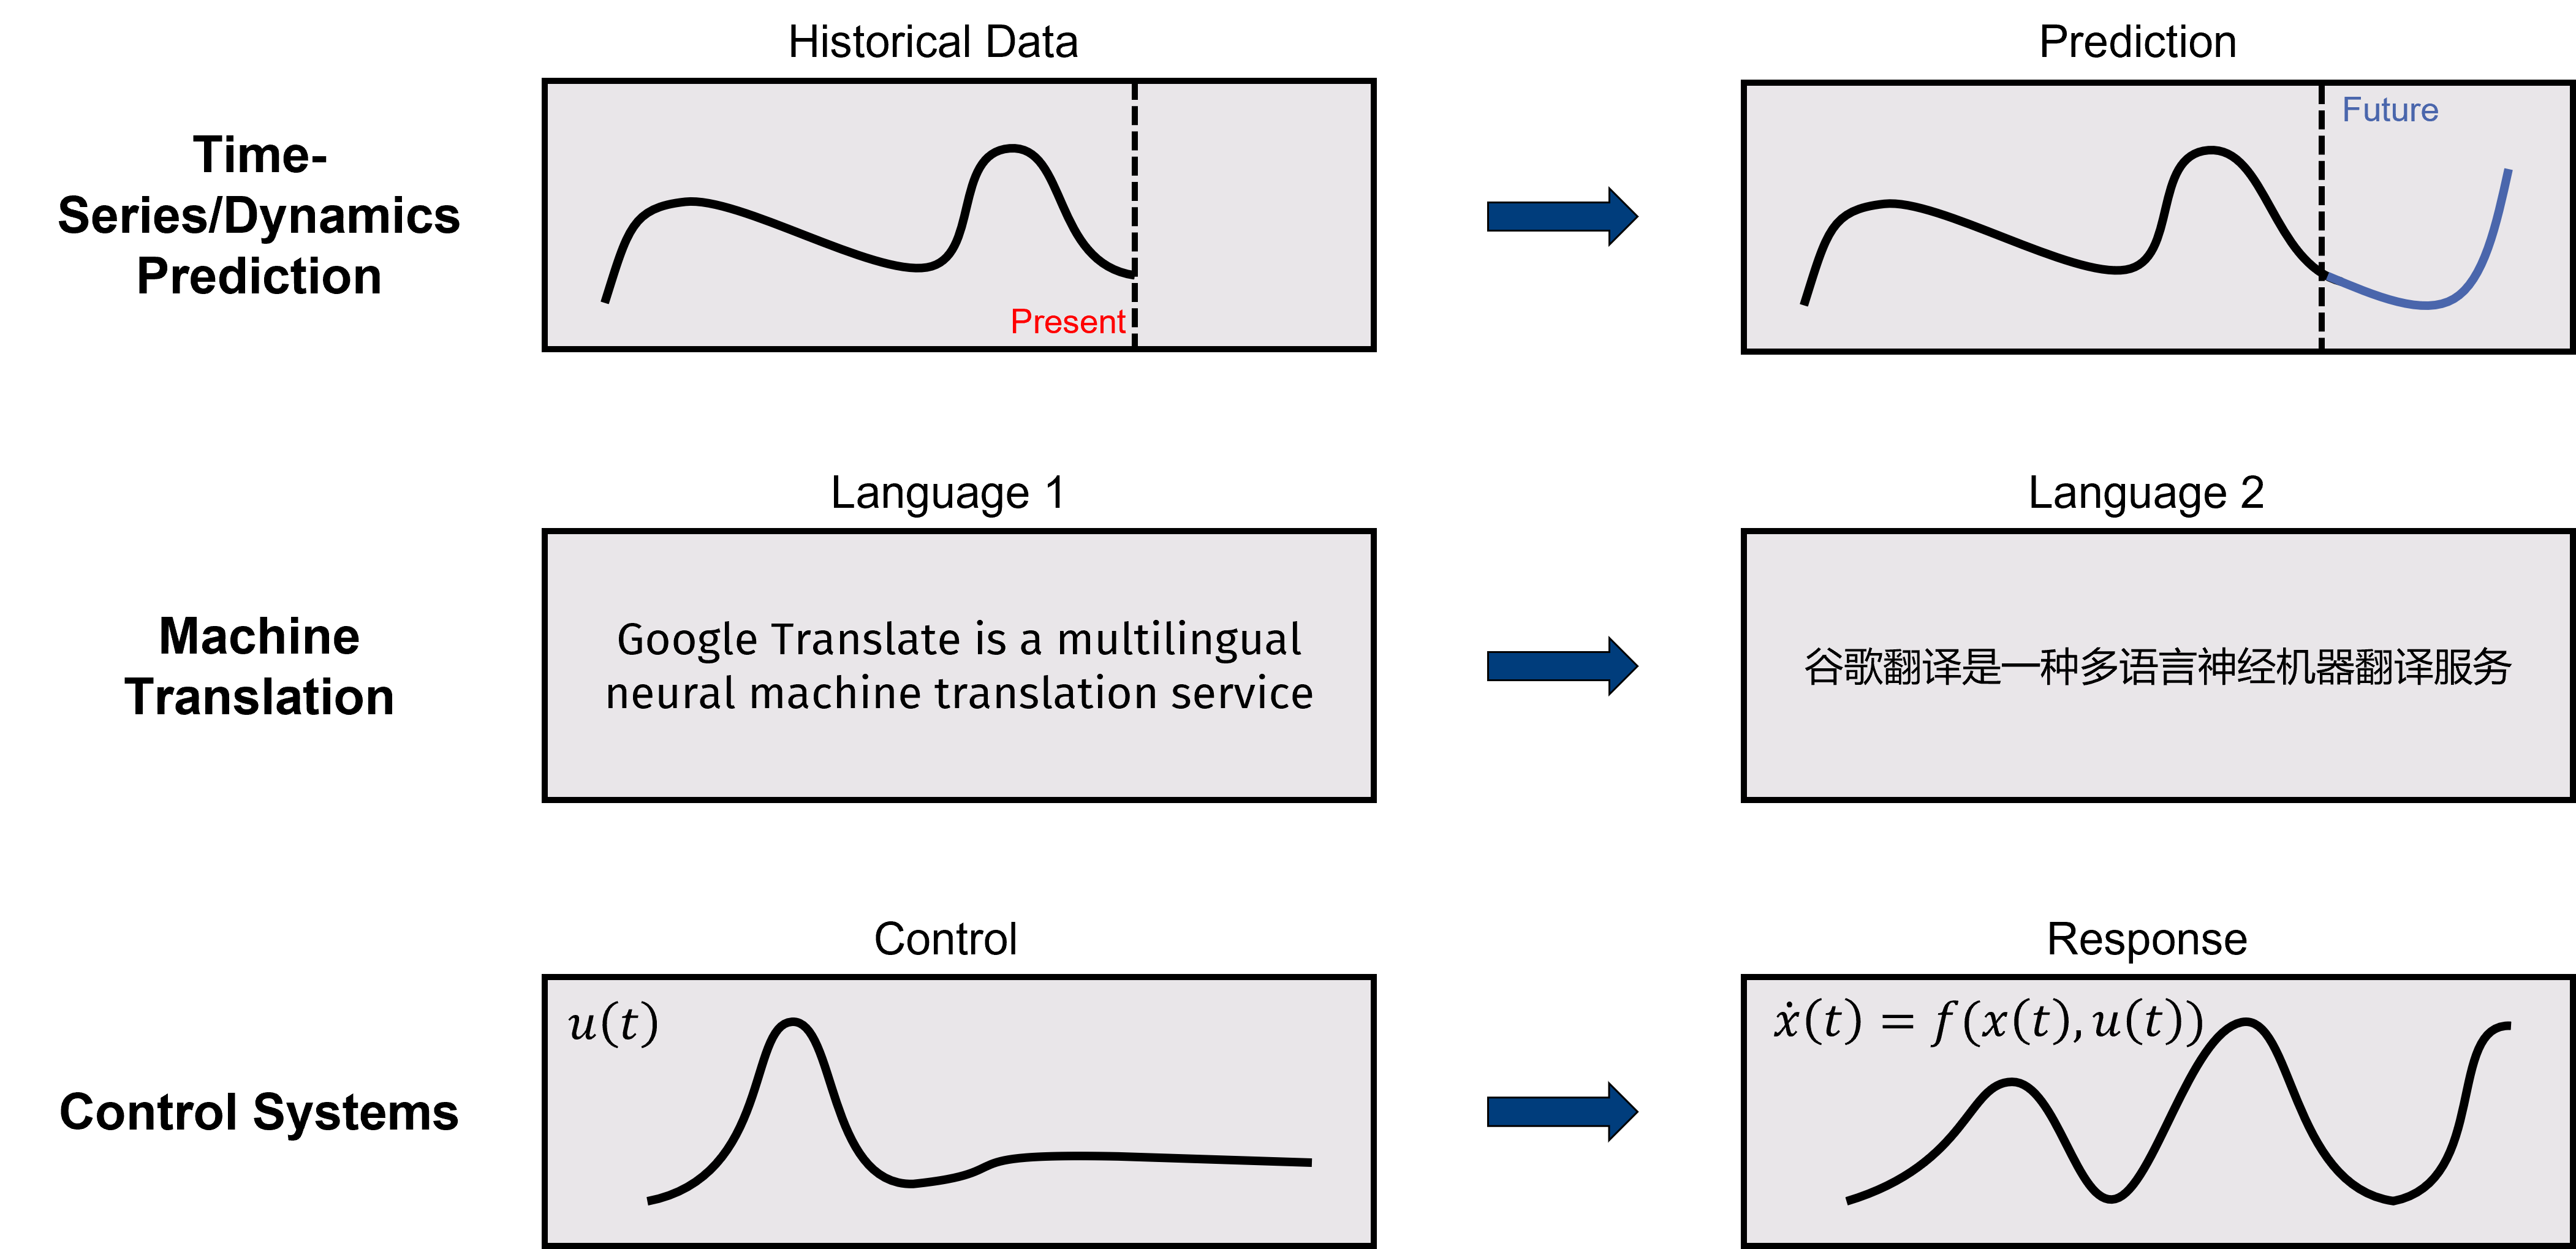
\includegraphics[width=\textwidth]{figures/seq_to_seq_applications.png}
    \end{center}

\end{frame}



\begin{frame}
    \frametitle{ML for DS: DL Architectures for Sequence Modelling}

    \begin{figure}
        \centering
        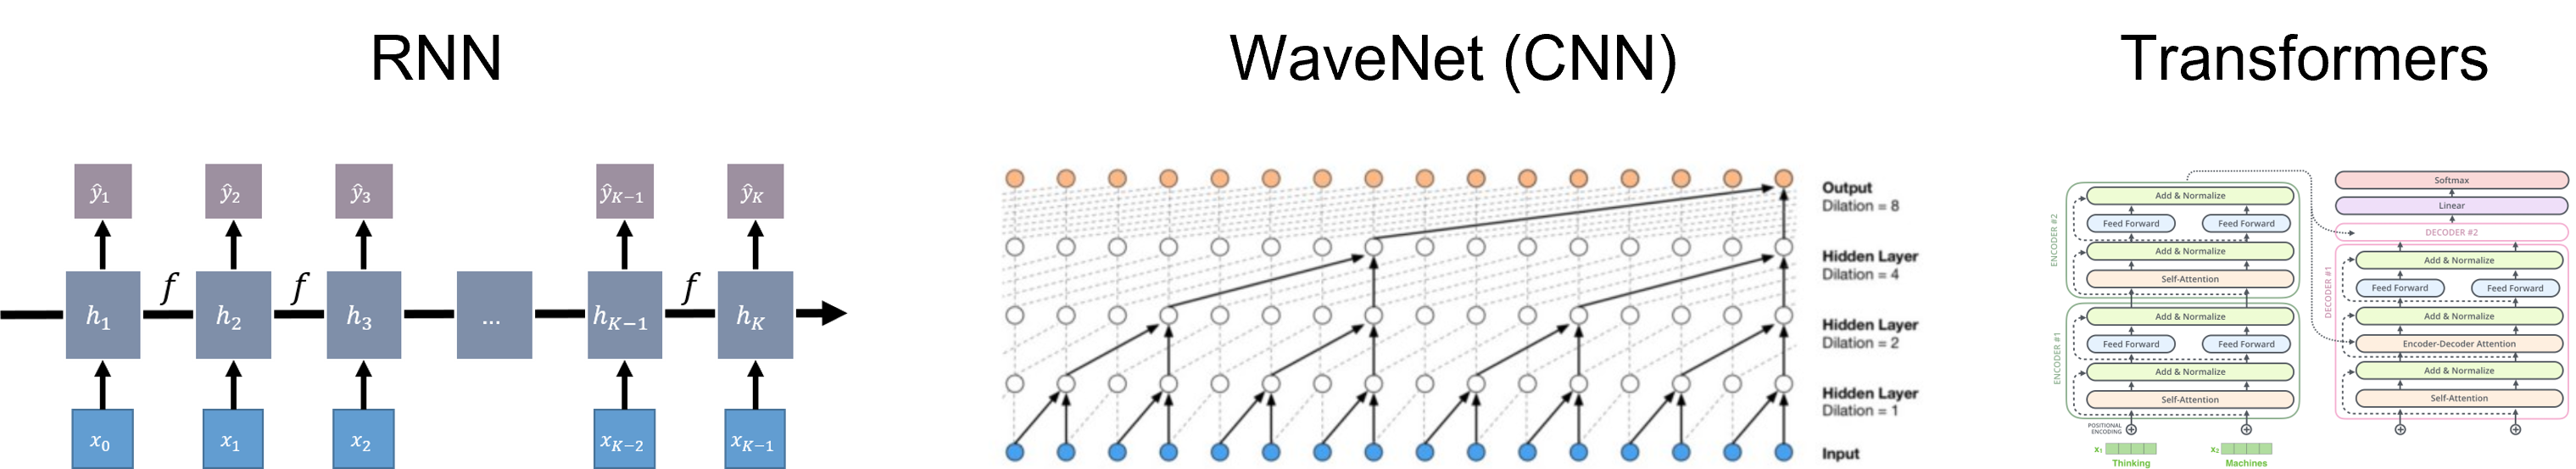
\includegraphics[width=\textwidth]{Figures/different_timeseries_archs.png}
    \end{figure}

    \begin{empheq}[box=\mymath]{gather*}
        \text{
            \textbf{General question:}
            How are they different? When should we use which?
        }
    \end{empheq}

\end{frame}

\begin{frame}
    \frametitle{Supervised Learning}

    \begin{center}
        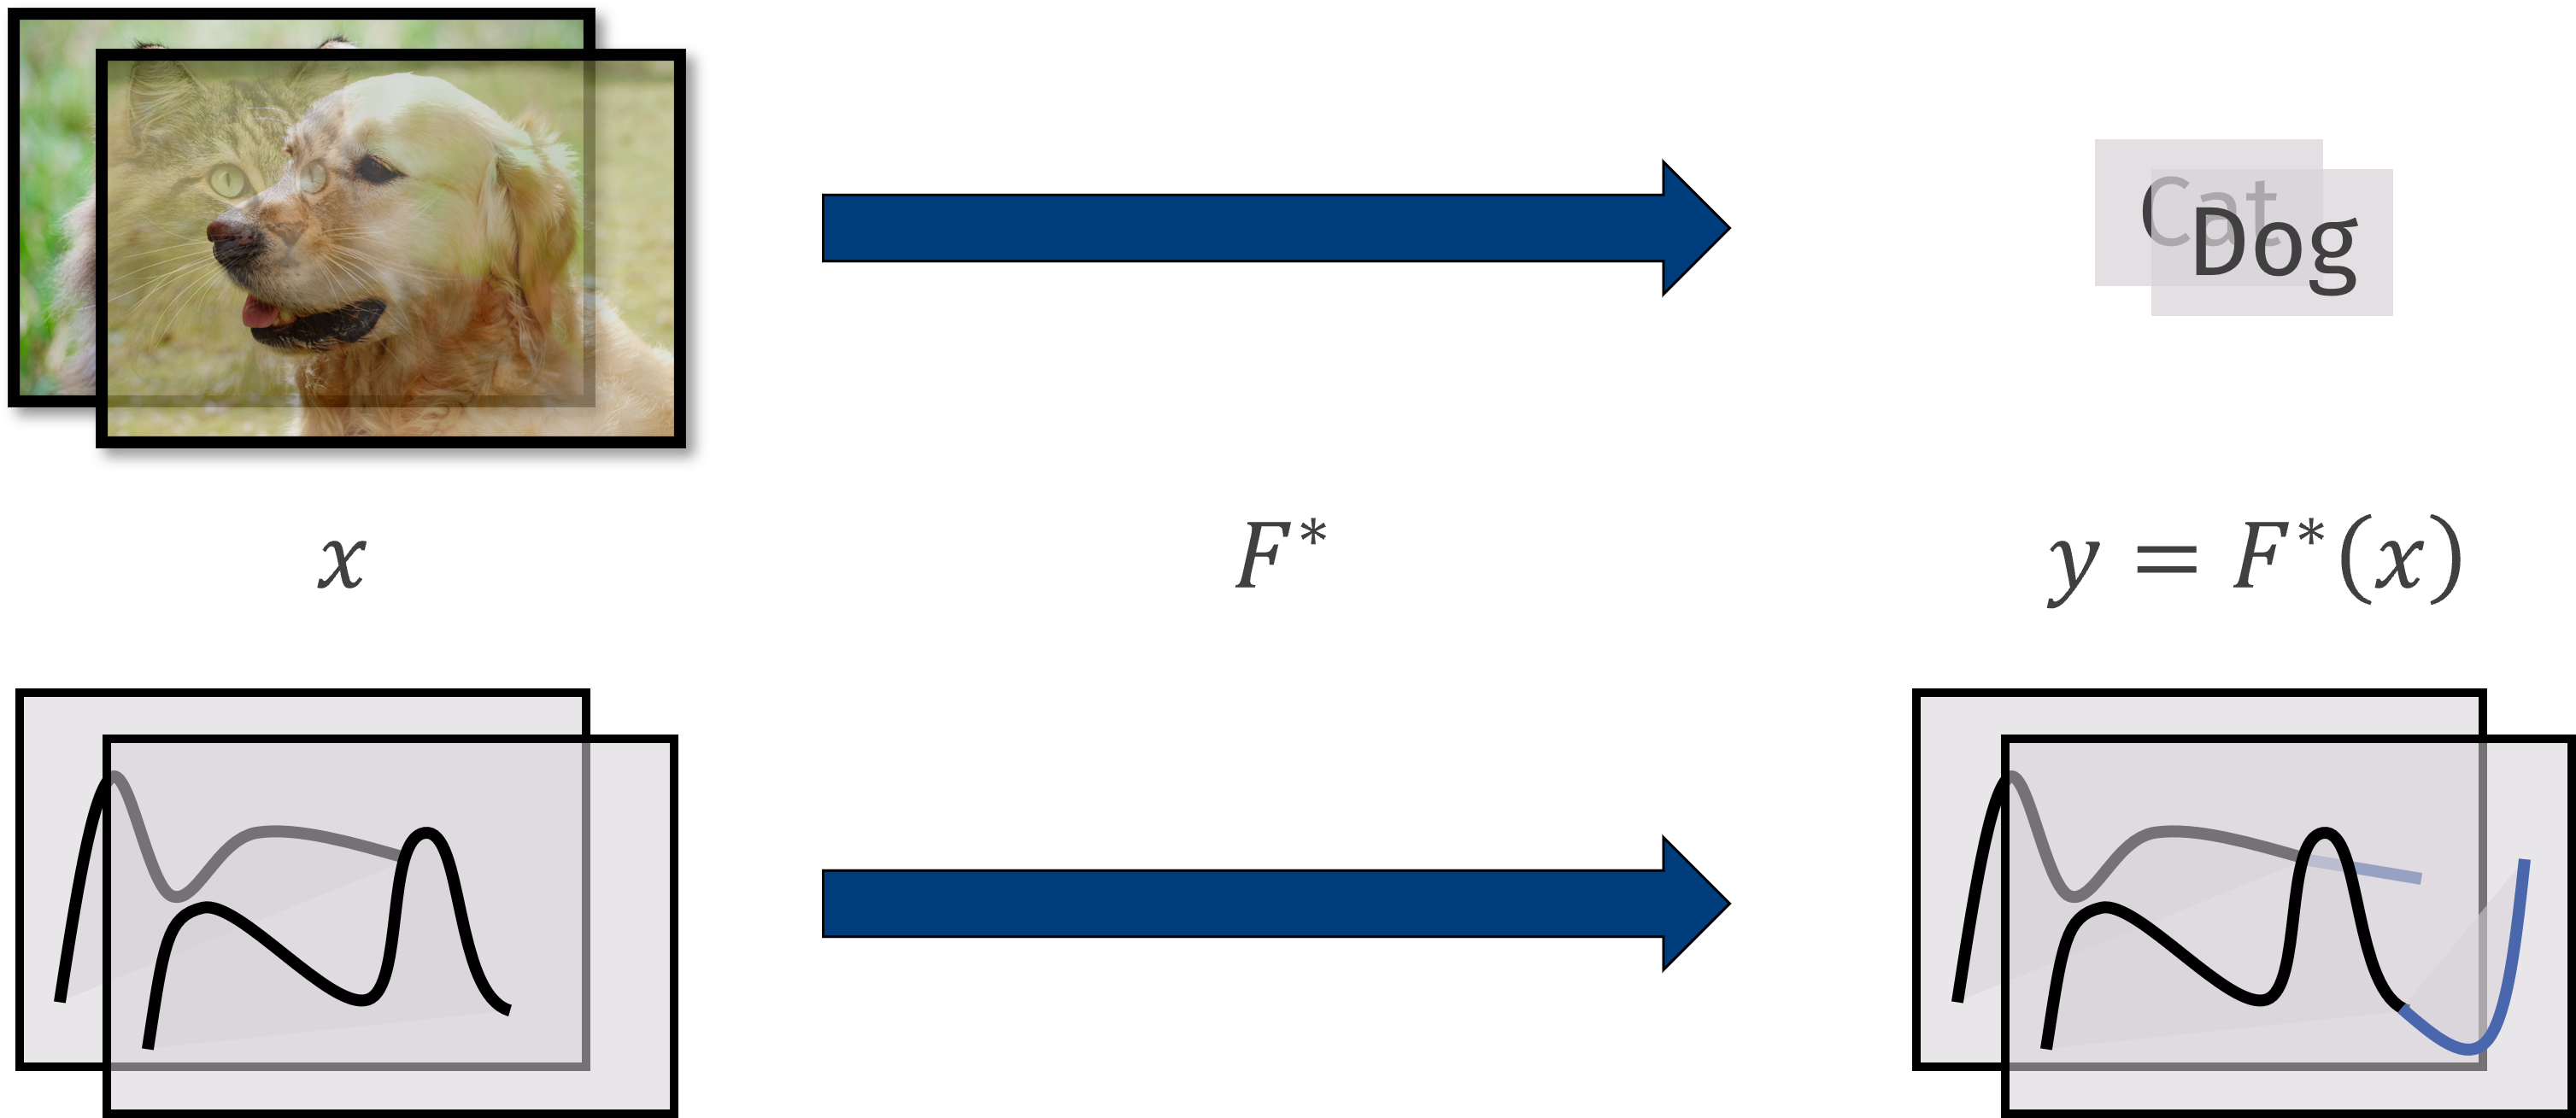
\includegraphics[width=0.8\textwidth]{Figures/target_function.png}
    \end{center}

    \pause{}

    \begin{empheq}[box=\mymath]{gather*}
        \text{
            \textbf{Goal:} Learn/approximate \alert{target} $F^*$
        }
    \end{empheq}


\end{frame}



\begin{frame}
    \frametitle{Modelling Static vs Dynamic Relationships}

    \begin{columns}[T] % align columns
        \begin{column}{.48\textwidth}
            {
                \color{nusorange}
                Static setting
                \rule{\linewidth}{4pt}
            }
            \begin{equation*}
                \begin{aligned}
                    &\text{\alert{(input)}}
                    \quad
                    &&x\in \Xcal = \R^d \\
                    &\text{\alert{(output)}}
                    \quad
                    &&y \in \Ycal = \R^n \\
                    &\text{\alert{(target)}}
                    \quad
                    &&y = F^*(x)
                \end{aligned}
            \end{equation*}
        \end{column}%
        \hfill%
        \pause{}
        \begin{column}{.48\textwidth}
            {
                \color{nusgreen}
                Dynamic setting
                \rule{\linewidth}{4pt}
            }
            \begin{equation*}
                \begin{aligned}
                    &\text{\alert{(input)}}
                    \quad
                    &&\*x = \{ x_k \in \R^d \} \in \Xcal
                    \\
                    &\text{\alert{(output)}}
                    \quad
                    &&\*y = \{ y_k \in \R^n \} \in \Ycal
                    \\
                    &\text{\alert{(target)}}
                    \quad
                    &&y_k = H_k^*(\*x) \quad \forall \quad k
                \end{aligned}
            \end{equation*}
        \end{column}%
    \end{columns}

    \vspace{.5cm}

    \pause{}

    Goal of supervised learning
    \begin{itemize}
        \item Static: learn/approximate $F^*$
        \item Dynamic: learn/approximate $\{ \Htar_k \}$
    \end{itemize}

\end{frame}


\begin{frame}
    \frametitle{Three Paradigms of Questions}

    \begin{overprint}
        \onslide<1>\centerline{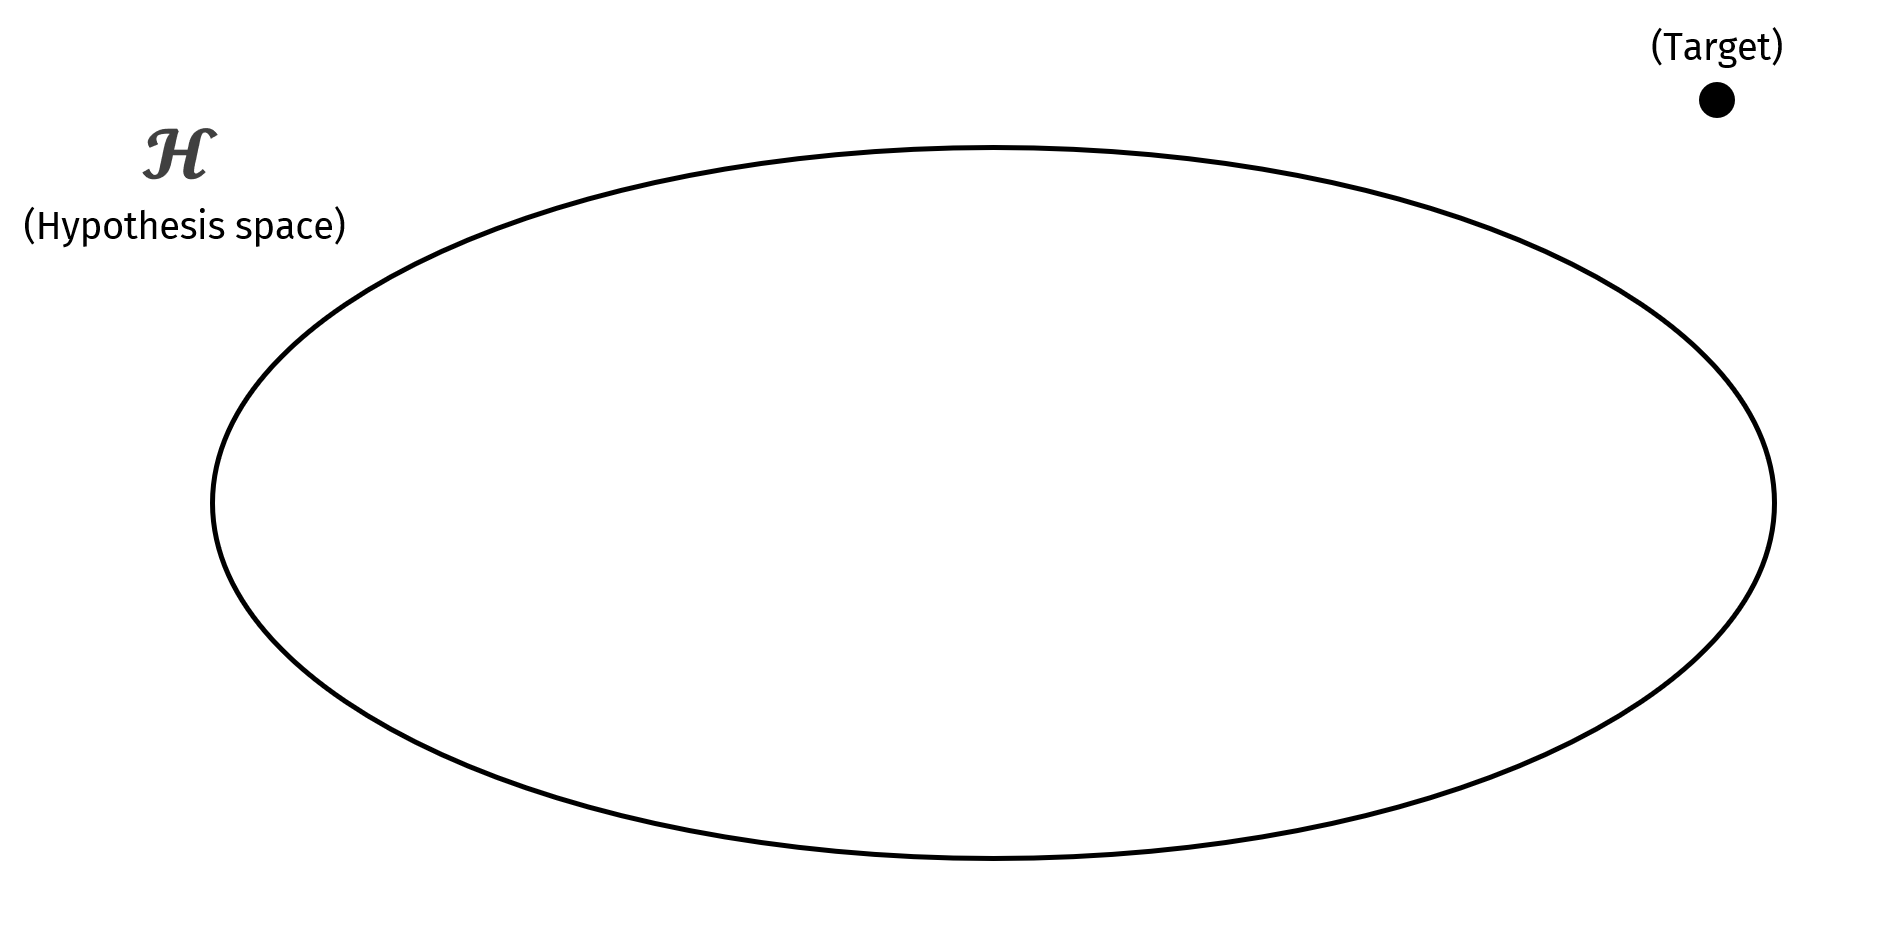
\includegraphics[width=\textwidth]{Figures/paradigm_1.png}}
        \onslide<2>\centerline{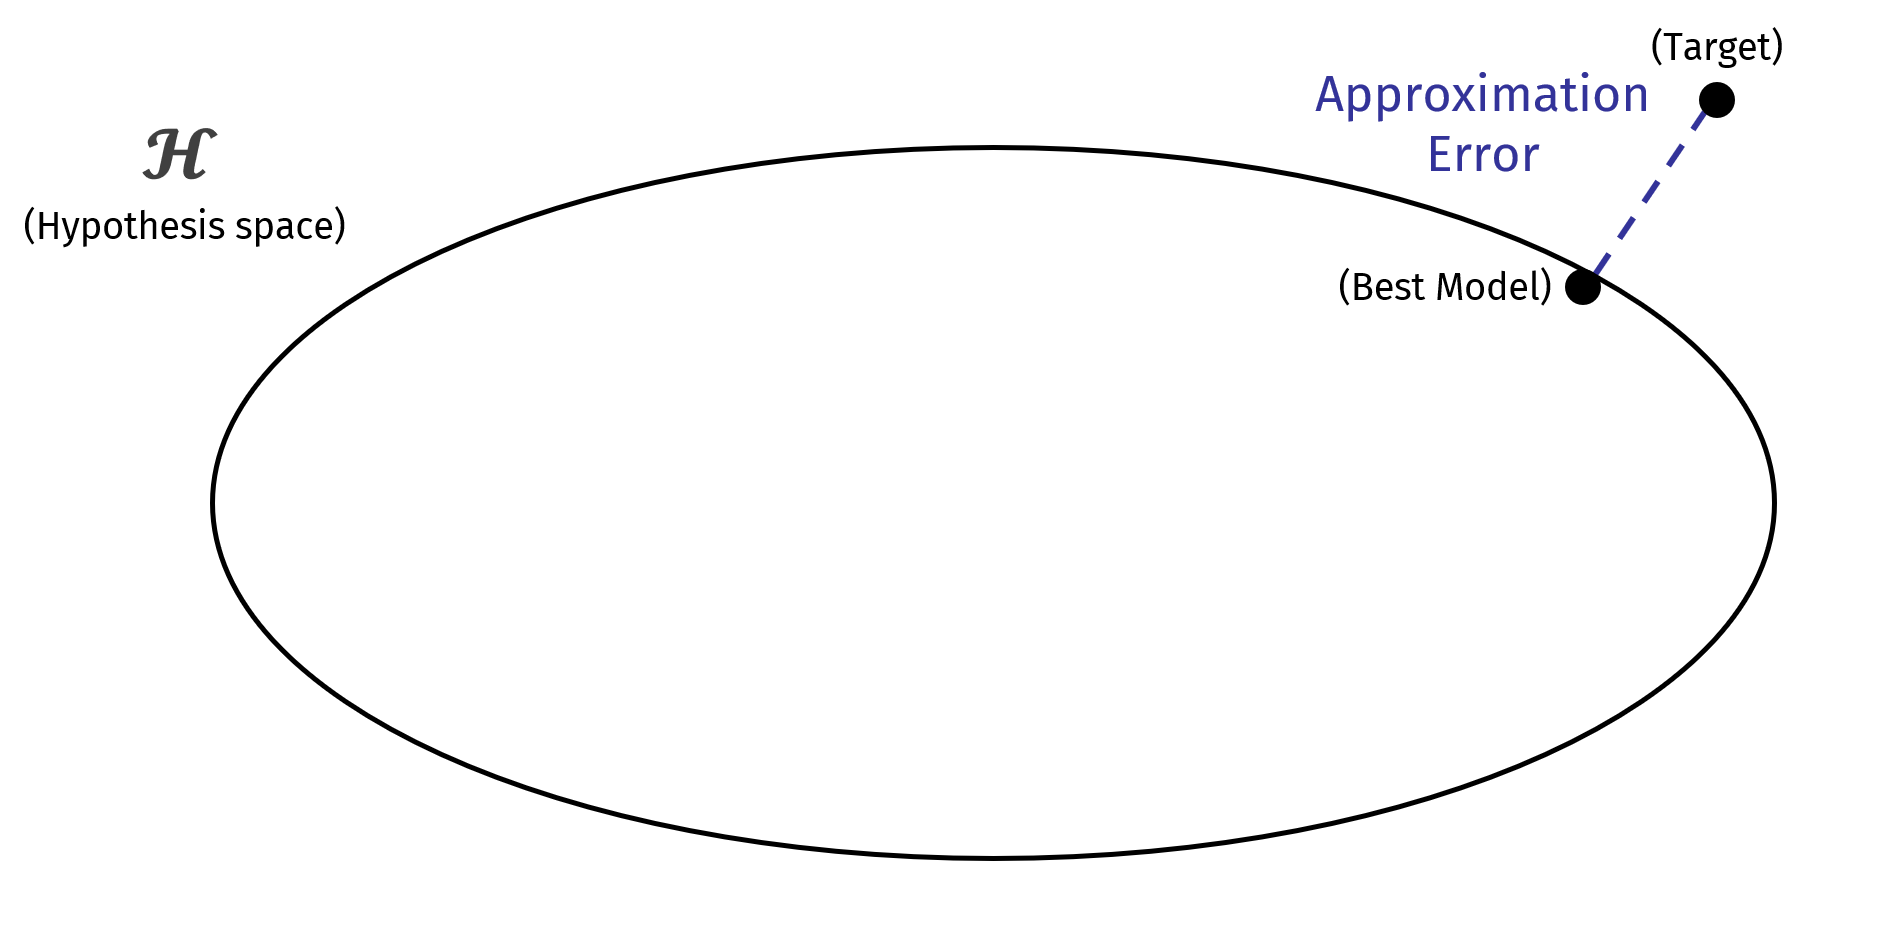
\includegraphics[width=\textwidth]{Figures/paradigm_2.png}}
        \onslide<3>\centerline{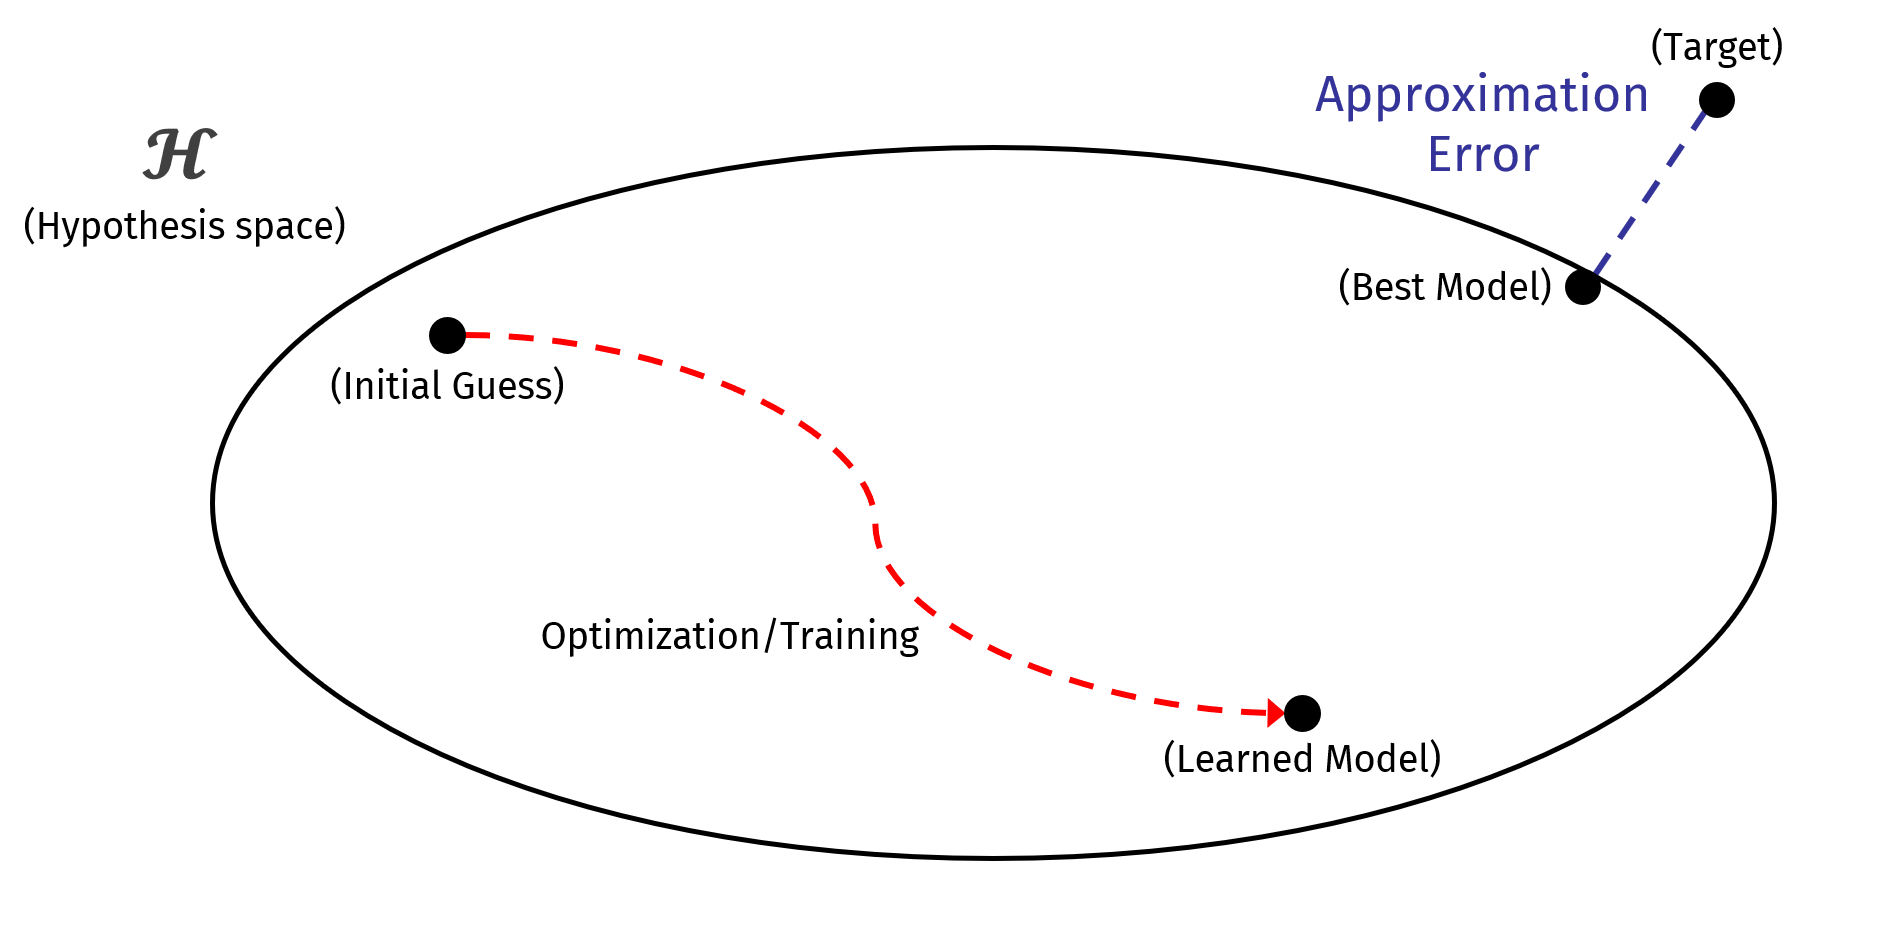
\includegraphics[width=\textwidth]{Figures/paradigm_3.png}}
        \onslide<4>\centerline{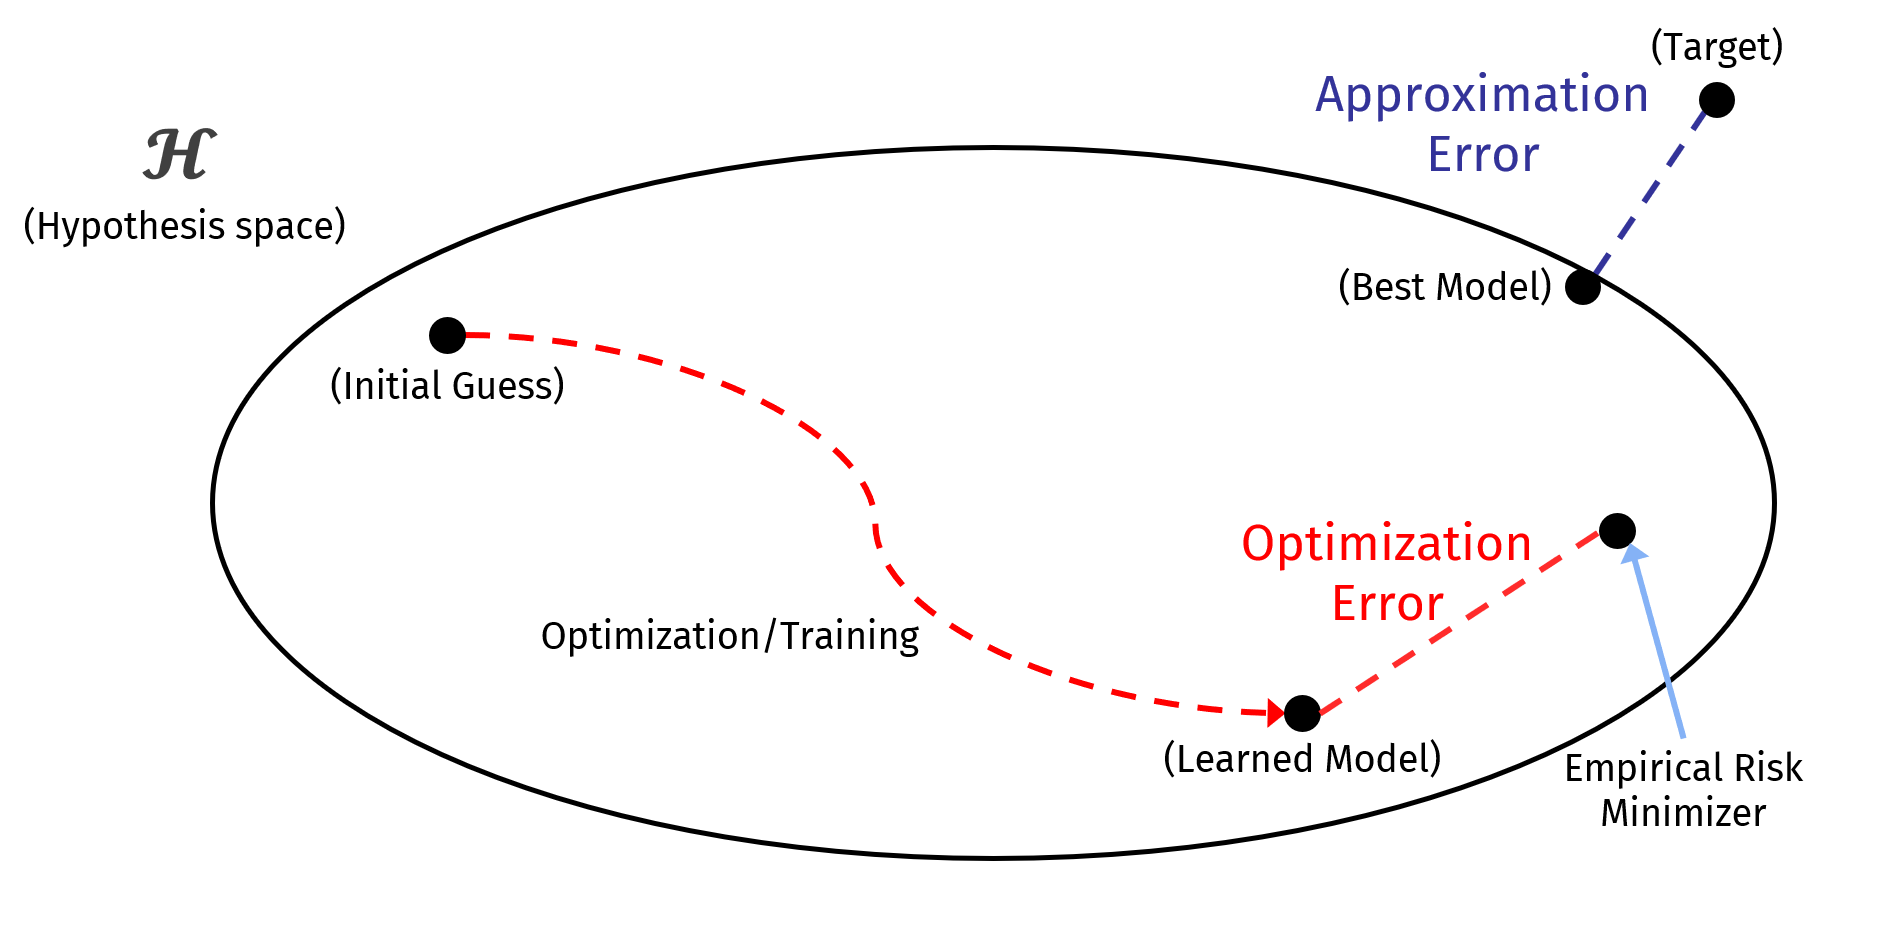
\includegraphics[width=\textwidth]{Figures/paradigm_4.png}}
        \onslide<5>\centerline{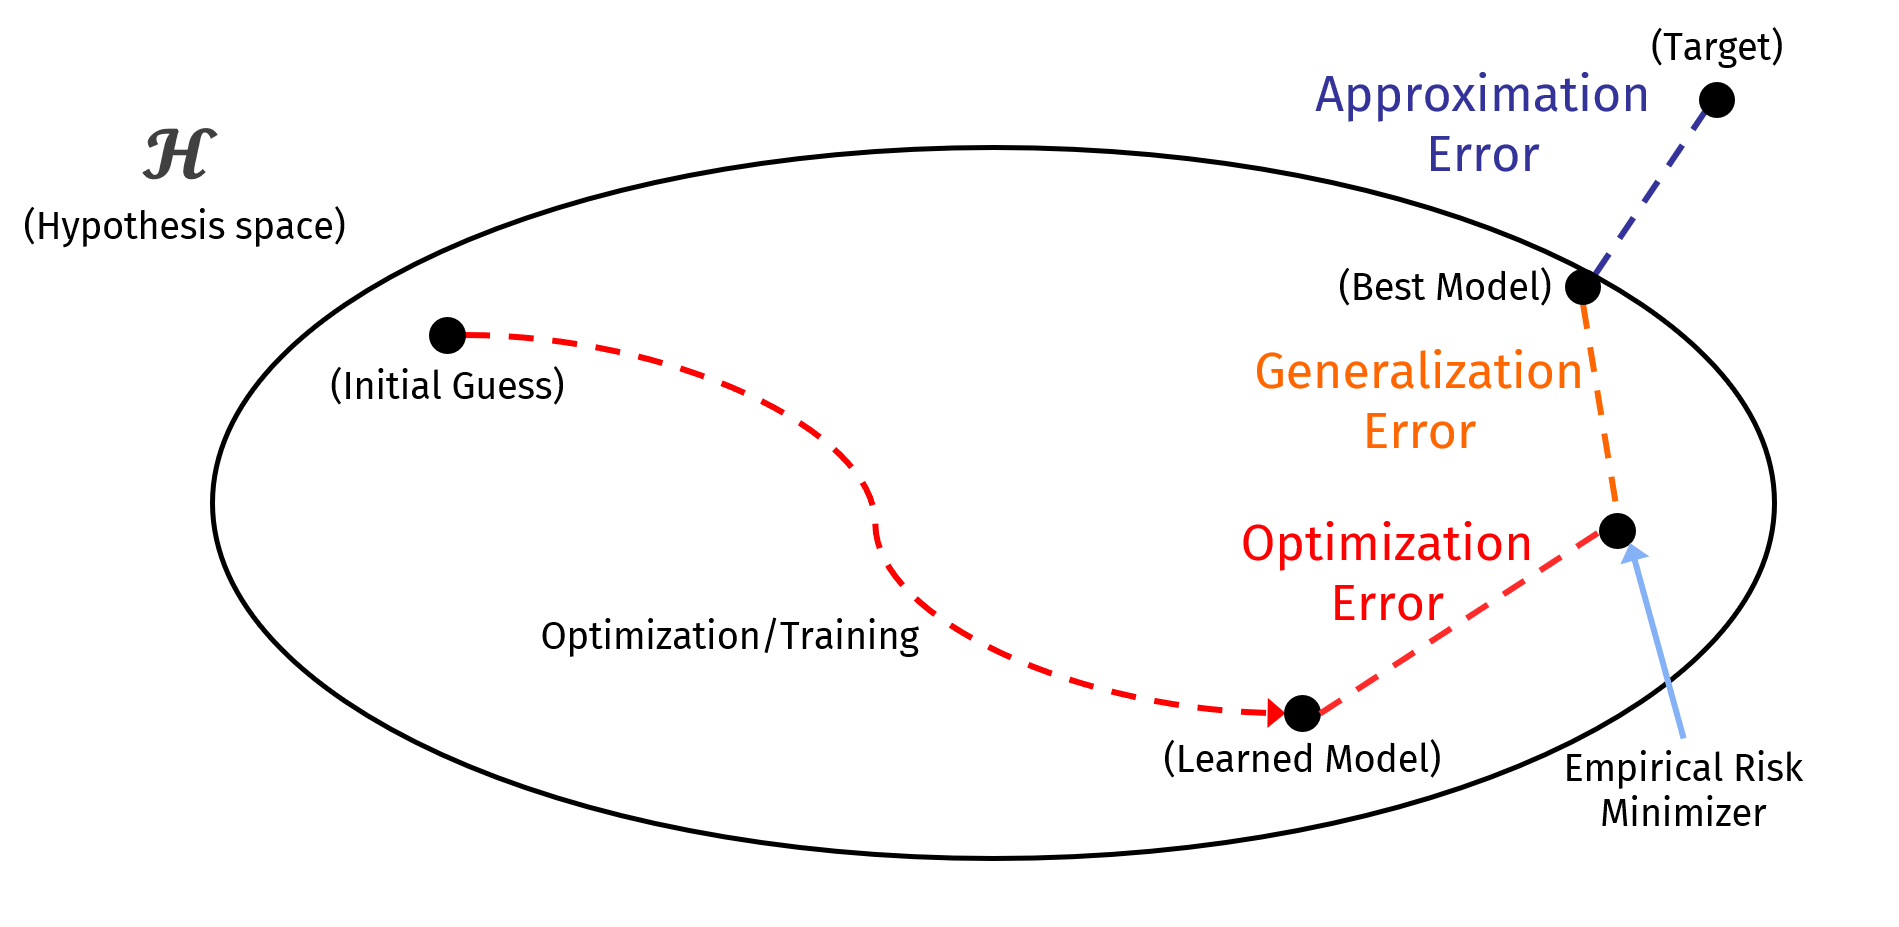
\includegraphics[width=\textwidth]{Figures/paradigm_5.png}}
    \end{overprint}
\end{frame}

\begin{frame}
    \frametitle{The Problem of Approximation}

    Given a hypothesis space $\Hcal$ and a target (concept) space $\Ccal$,
    we seek two types of approximation results
    \begin{itemize}
        \item Universal Approximation (Density)
        \begin{empheq}[box=\mymath]{gather*}
            \text{
                For each $H^* \in \Ccal$ and $\epsilon>0$, there exist $\wh{H} \in \Hcal$
                such that $\Vert H^* - \wh{H} \Vert \leq \epsilon$
            }
        \end{empheq}
        \pause{}
        \item Approximation Rates.
        Let ${\Hcal} = \cup_{m} {\Hcal}_{m}$,
        where ${\Hcal}_{m} \subset {\Hcal}_{m+1}$,
        $m$ measures size of hypothesis space (approximation budget)
        \begin{empheq}[box=\mymath]{gather*}
            \text{
                $
                    \inf_{\wh{H} \in {\Hcal}_m}
                    \Vert H^* - \wh{H}  \Vert
                    \leq
                    \text{Complexity}(H^*) \text{rate}(m)
                $,
                \qquad
                $\text{rate}(m) \rightarrow 0$
            }
        \end{empheq}
    \end{itemize}

\end{frame}

\begin{frame}
    \frametitle{Example: Approximation by Trigonometric Polynomials}

    Consider
    \begin{itemize}
        \item
        $\Ccal = C^{\alpha}_{\text{per}}([0,2\pi], \R)$ (periodic $C^{\alpha}$ functions)
        \item
        $
            {\Hcal}_m
            =
            \left\{
                \sum_{i=0}^{m-1} a_i \cos(i x) + b_i \sin(i x)
                :
                a_i,b_i \in \R
            \right\}
        $
        (trigonometric polynomials)
    \end{itemize}
    \pause{}
    Then, for each $H^* \in \Ccal$ \refhl{[Jackson, 1930]}
    \begin{equation*}
        \inf_{\wh{H} \in \Hcal_m}
        \| H^* - \wh{H} \|_{C}
        \leq
        \frac{C(\alpha)\max_{i\leq \alpha}\| {H}^{*(i)}\|_C}{m^\alpha}
    \end{equation*}
    Here, $\text{Complexity}(H^*) = \max_{i\leq\alpha} \| H^{*(i)} \|_C$
    and
    $\text{rate}(m) = m^{-\alpha}$.

    \pause{}
    \begin{empheq}[box=\mymath]{gather*}
        \text{
            \textbf{Insight:}
            Efficient approximation if $H^*$ is smooth (small gradient norm)
        }
    \end{empheq}
\end{frame}

\begin{frame}
    \frametitle{An Approximation Theory for Sequence Modelling}

    Our goal is to derive similar statements like Jackson's Theorem, but for
    \begin{itemize}
        \item $\Ccal$ $\rightarrow$ suitable classes of sequence relationships (functionals)
        \item $\Hcal$ $\rightarrow$ RNNs, CNNs/WaveNets, Encoder-Decoders, Transformers
    \end{itemize}

    \pause{}

    For each case, we aim to characterize
    \begin{itemize}
        \item What $\Ccal$ can be approximated (efficiently)?
        \item How does the complexity measure and rate estimate depend on different ${\Hcal}$?
        \item How to choose which $\Hcal$ to use in practice?
    \end{itemize}


\end{frame}

    \section{Recurrent Neural Networks}


\begin{frame}
	\frametitle{The Recurrent Neural Network Hypothesis Space}
	The \alert{recurrent neural network (RNN)} architecture
	% \setlength{\leftmargini}{0.5em}
	\begin{columns}
		\begin{column}[T, onlytextwidth]{.45\textwidth}%
		\setlength{\partopsep}{0pt}%
		\begin{equation*}
			\begin{aligned}
			h_{k+1} &= \sigma(Wh_{k} + Ux_{k}),
			\qquad h_k \in \R^m
			% \qquad k=0,1,\dots,K-1
			\\
			h_0 &= 0
			\\
			\wh{y}_k &= c^\tp h_{k}
			\end{aligned}
		\end{equation*}
		\end{column}%
		\begin{column}[T]{.45\textwidth}
		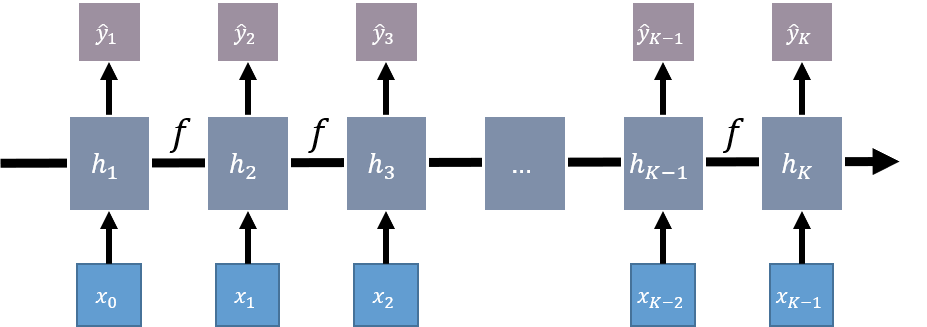
\includegraphics[width=\textwidth]{figures/recurrent_structure.png}
		\end{column}%
	\end{columns}

	\vspace{.5cm}

	\pause{}


    \begin{itemize}[<+->]
        \item
        The RNN parametrizes a sequence of functions
        $
            \{
            \wh{H}_k
            =
            \{x_0,\dots,x_{k-1}\} \mapsto \wh{y}_k
            \}.
        $
        \item
        A continuous-time idealization parametrizes functionals
        $\{ \*x \equiv \{x_t\} \mapsto \wh{y}_t \}$
        \begin{equation*}
            \dot{h}_t = \sigma(Wh_t + Ux_t),
            \quad h_{-\infty} = 0,
            \quad \wh{y}_t = c^\tp h_t,
            \quad t \in \R
        \end{equation*}
        \item
        Note: this is different from the dynamical viewpoint on deep neural networks,
        where the considered mapping is the flow map $h_0 \mapsto h_T$ \refhl{[E, 2017]}.
        Approximation theory: \refhl{[LLS, 2022]}

    \end{itemize}

    {\only<4->{
            \blfootnote{
                \fullcite{li2022deep}
            }
        }
    }
\end{frame}

\begin{frame}[focus]
    Empirically, it is found RNN performs poorly when modelling \\
	``long-term memory''

    \medskip

    Can we investigate this phenomena precisely?
\end{frame}


\begin{frame}
    \frametitle{The Linear RNN Hypothesis Space}

	We analyze the linear case where $\sigma(h) = h$, we have the dynamics
    \begin{equation*}
        \begin{split}
            \begin{aligned}
                \wh{y}_t &= c^\top h_t, \\
                \dot{h}_t &= W h_t + U x_t.
            \end{aligned}
        \end{split}
        \qquad
        \text{where}
        \qquad
        \begin{split}
            \begin{aligned}
                &h_t \in \R^m
                & & \text{(hidden state)}
                \\
                &W \in \R^{m \times m}
                & & \text{(Recurrent Kernel)}
                \\
                &U \in \R^{m \times d}
                & & \text{(Input Kernel)} \\
                &c \in \R^{m}
                & & \text{(Output layer weights)}
            \end{aligned}
        \end{split}
    \end{equation*}

    \pause{}

    This gives rise to the (stable) linear RNN hypothesis space

	\small
    \begin{empheq}[box=\mymath]{gather*}
        \hrnn =
        \cup_{m\geq 1}
        \underbrace{
            \left\{
                \{\wh{H}_t(\*x), t\in\R \} : \wh{H}_t(\*x) = \int_{0}^{\infty} c^\tp e^{Ws} U x_{t-s} ds,
                W \in \Wcal_m, U\in\R^{m\times d}, c \in \R^{m}
            \right\}
        }_{\hrnn^{(m)}}\\
        \Wcal_m = \{ W \in \R^{m\times m} : \text{eigenvalues of $W$ have negative real parts (Hurwitz)} \}
    \end{empheq}
	\normalsize
\end{frame}

\begin{frame}
    \frametitle{Properties of Linear RNN Hypothesis Space}

    \begin{empheq}[box=\mymath]{gather*}
        \hrnn^{(m)} =
        \cup_{m\geq 1}
		\left\{
			\{ \wh{H}_t(\*x) = \int_{0}^{\infty} c^\tp e^{Ws} U x_{t-s} ds \}
			:
			W \in \Wcal_m, U\in\R^{m\times d}, c \in \R^{m}
		\right\}
    \end{empheq}

    \begin{alertblock}{Proposition}
        Let $\{ \wh{H}_t : t\in\R \}$ be any family of functionals in $\hrnn$.
        Then for each $t\in\R$,
        \begin{itemize}
            \item $\wh{H}_t$ is a continuous, linear functional.
            \item $\wh{H}_t$ is a causal functional.
            \item $\wh{H}_t$ is a regular functional.
            \item The family $\{ \wh{H}_t : t\in\R\}$ is time-homogeneous.
        \end{itemize}
    \end{alertblock}

\end{frame}


\begin{frame}
	\frametitle{Approximation Guarantee (Density)}

	\begin{alertblock}{Theorem [LHEL, 2021]}
		Let $\{ \Htar_t : t\in\R \}$ be a family of continuous, linear, causal,
        regular and time-homogeneous functionals on $C_0(\R,\R^d)$.
        Then, for any $\epsilon > 0$ there exists $\{ \wh{H}_t : t\in \R \} \in \hrnn$ such that
		\begin{equation*}
            \| {\bm H^*} - {\wh{\bm H}} \|
            \equiv
			\sup_{t\in\R}
			\sup_{\| \*x \|_C \leq 1}
			|
			\Htar_t(\*x) - \wh{H}_t(\*x)
			|
			\leq \epsilon.
		\end{equation*}
	\end{alertblock}

	Main idea: Prove a general Riesz representation
	\begin{equation*}
		H^*_t(\*x) =
		\int_{0}^{\infty}
        \rho(s)^\tp
		x_{t-s}
		ds
        \qquad
        \alert{
            \left[
                \text{Recall: }
                \wh{H}_t(\*x) = \int_{0}^{\infty} c^\tp e^{Ws} U x_{t-s} ds
            \right]
        }
	\end{equation*}
	Then, RNN approximation reduces to the $L^1$ approximation of $\rho(t)$ by $[c^\tp e^{Wt} U]^\tp$.

	\blfootnote{
		\fullcite{li2020onthe}
	}

\end{frame}


\begin{frame}
    \frametitle{Smoothness and Memory}

	Approximation rates depend on appropriate complexity measures

    \pause{}

    Key concepts: \alert{smoothness} and \alert{memory}

    \begin{figure}
        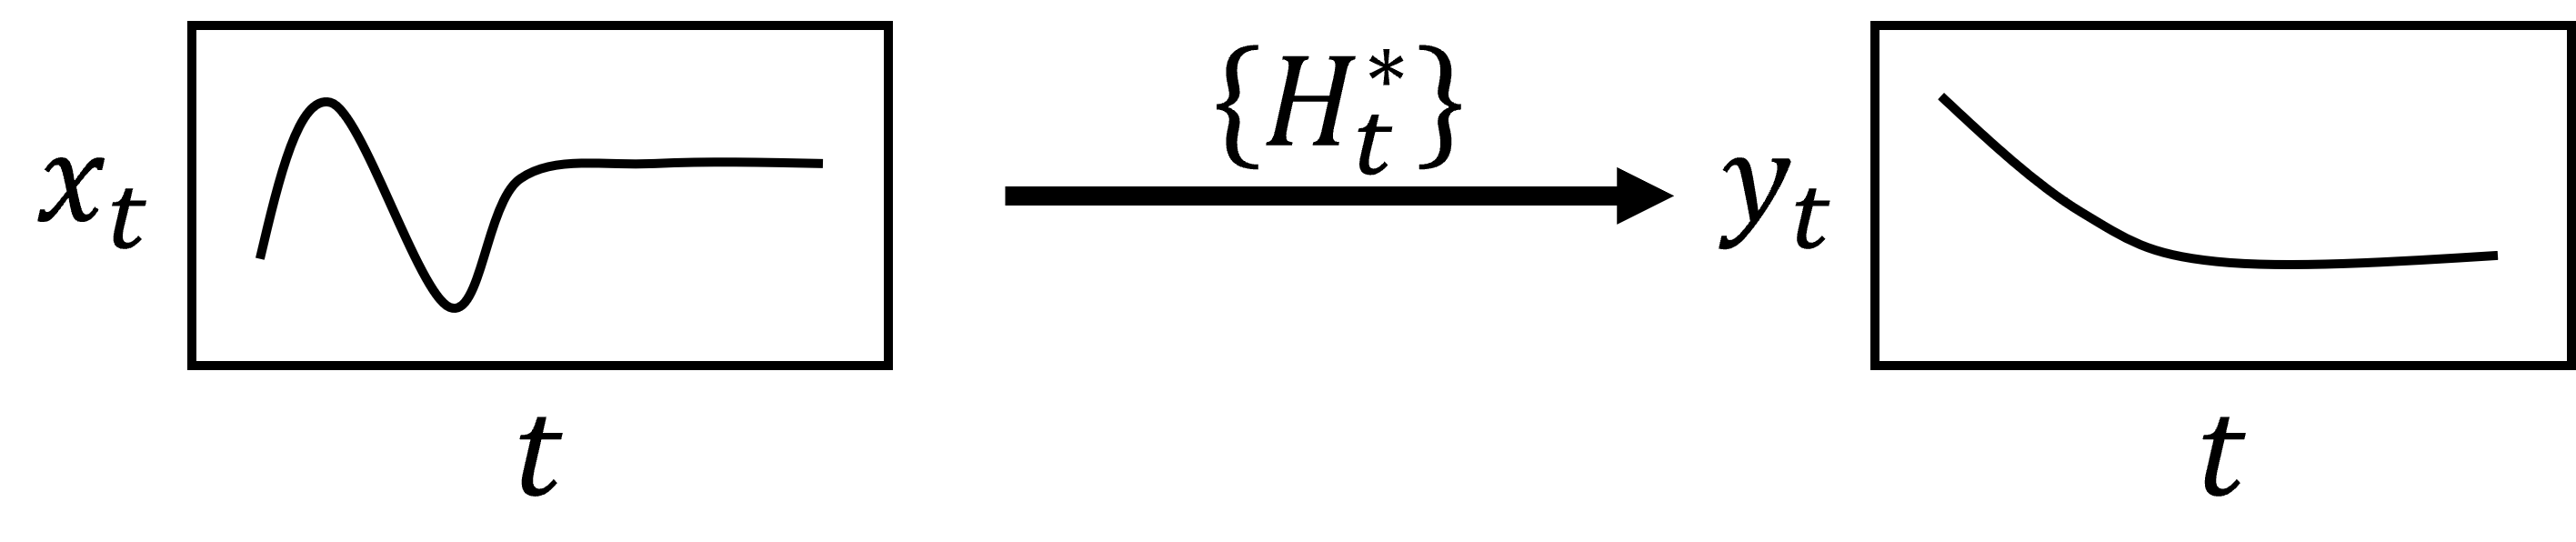
\includegraphics[width=0.48\textwidth]{figures/easy_approx.png}
        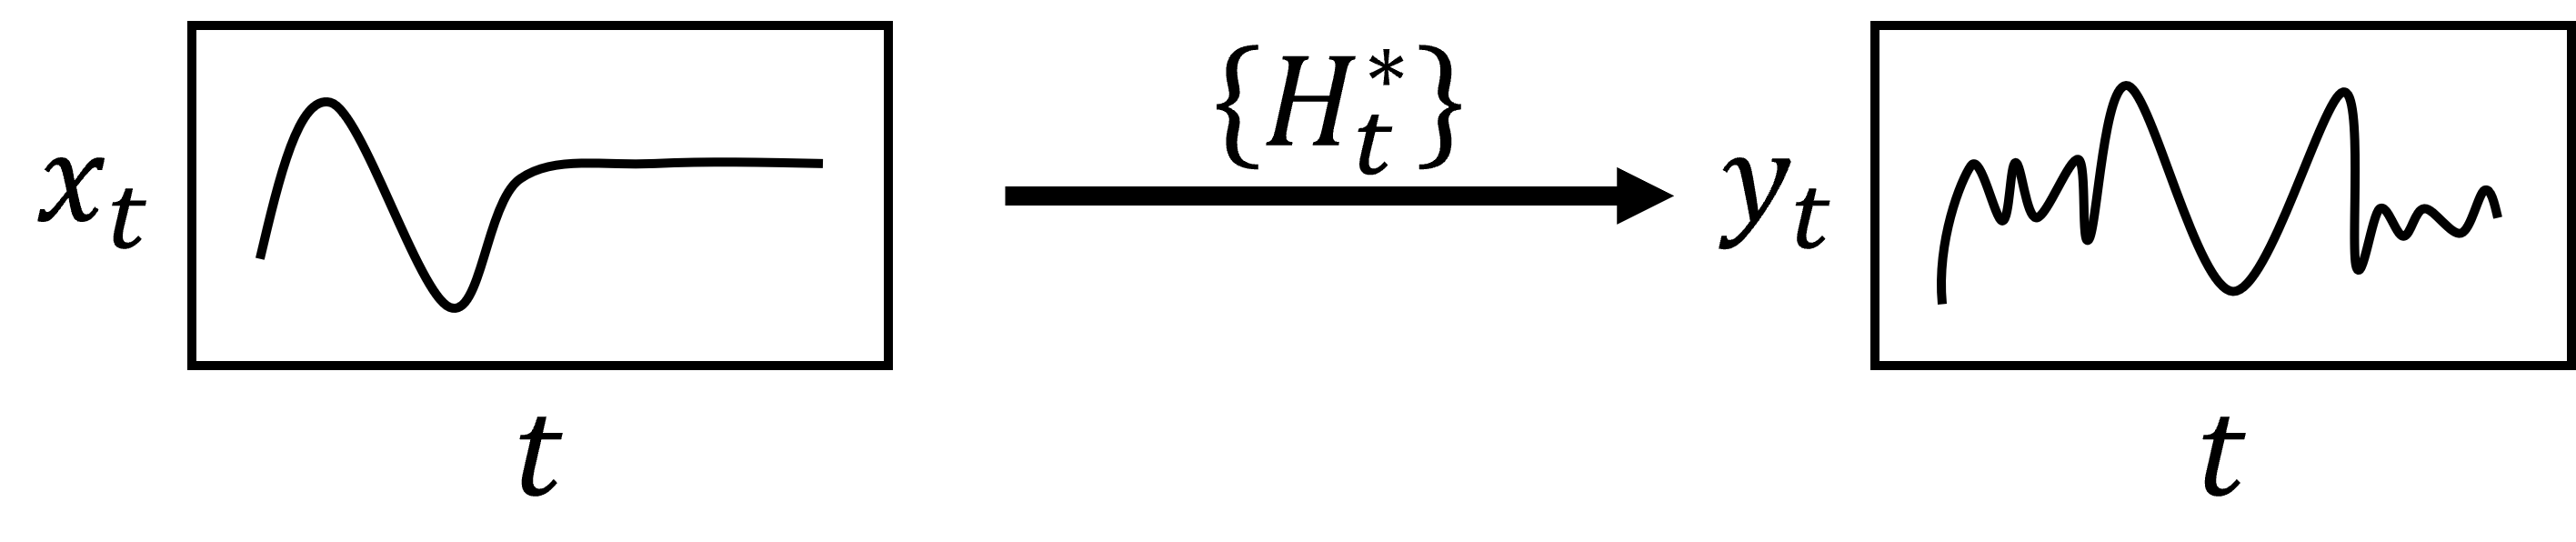
\includegraphics[width=0.48\textwidth]{figures/hard_approx.png}
    \end{figure}

    \pause{}

    Define
    \begin{itemize}
        \item $e_i$, $i=1,\dots,d$ as the standard basis vectors in $\R^d$
        \item $\*e_i$ as the constant signal $e_{i,t} = e_i \ind_{\{t\geq 0\}}$
    \end{itemize}

    \pause{}

    Given a family of functionals $\{\Htar_t : t\in\R\}$
    \begin{itemize}
        \item Denote the output of constant signal $y_i(t) := \Htar_t(\*e_i)$
        \item \alert{smoothness} is characterized by the smoothness of $t\mapsto y_i(t)$
        \item \alert{memory} is characterized by the decay rate of the $t\mapsto y_i^{(k)}(t)$
    \end{itemize}
\end{frame}


\begin{frame}
    \frametitle{Approximation Rate}

    \begin{alertblock}{Theorem [LHEL, 2021]}
        Set $y_i = H^*_t(\bm e_i)$.
        Suppose there exist constants $\alpha\in \Z^+, \beta,\gamma\in \R^+$
        such that for $i=1,\dots,d$, $y_i(t) \in C^{(\alpha+1)}(\R)$ and for $k=1,\dots,\alpha+1$,
        \begin{equation*}
            e^{\beta t}y_i^{(k)}(t) = o(1) \text{ as } t \rightarrow +\infty
            \qquad
            \text{and}
            \qquad
            \sup_{t \geq 0} \frac{ |e^{\beta t}y_i^{(k)}(t)|}{\beta^k} \leq \gamma.
        \end{equation*}
        Then there exists a universal constant $C(\alpha)$ such that for each $m \geq 1$,
        % there exists $\{\wh{H}_t\} \in \wh{\Hcal}_m$ such that
        \begin{equation*}
            \inf_{\wh{\bm H} \in \hrnn^{(m)}}
            \| \bm \Htar - \wh{\bm H} \|
            % \sup_{t\in\R}
            % \| \Htar_t - \wh{H}_t \|
            % \equiv
            % \sup_{t\in\R}
            % \sup_{\| \*x \|_C \leq 1}
            % |
            %     \Htar_t(\*x) - \wh{H}_t(\*x)
            % |
            \leq \frac{C(\alpha)\gamma d}{ \beta m^\alpha}.
        \end{equation*}
    \end{alertblock}

    \blfootnote{
        \fullcite{li2020onthe}
    }
\end{frame}

\begin{frame}
	\frametitle{Curse of Memory in Approximation}

    Rate estimate
    \begin{equation*}
        \inf_{\wh{\bm H} \in \hrnn^{(m)}}
        \| \bm \Htar - \wh{\bm H} \|
        % \sup_{t\in\R}
        % \|
        %     H^*_t - \wh{H}_t
        % \|
        \leq \frac{C(\alpha)\gamma d}{ \beta m^\alpha}.
    \end{equation*}

    \pause{}

    Observations
    \begin{itemize}[<+->]
        \item The smoothness dependence ($\alpha$) is what one would expect in approximation theory
        \item The memory dependence ($\beta,\gamma$) is new:
        assumption means the temporal derivatives of
        $y_i(t) \equiv \Htar_t(\*e_i)$ must decay like $e^{-\beta t}$ for some $\beta>0$
        \item There is no curse of dimensionality - this is because we are in a linear setting,
        so dimensions can be separated in a linear fashion
        \item However, hidden in these results is a \alert{curse of memory}.
        A truncation argument shows that
    \end{itemize}

    {\onslide<5>
        \begin{empheq}[box=\mymath]{align*}
            \text{If $H^*_t(\*e_i) \sim t^{-\omega}$},
            \text{ then to get error $\epsilon$, need }
            m \sim
            \mathcal{O}
            \left(
                \omega \varepsilon^{-\frac{1}{\omega}}
            \right)
        \end{empheq}
    }
\end{frame}

\begin{frame}
	\frametitle{Insights on the (Linear) RNN Hypothesis Space}

    \begin{empheq}[box=\mymath]{gather*}
        \text{
            \textbf{Insight:}
            Efficient approximation if ${\bm H^*}$ is smooth
        } \\
		\text{
			and has exponential decaying memory
		}
    \end{empheq}

	Futhermore
	\begin{itemize}
		\item The ``only if'' part is also true \refhl{[LHEL, 2022]}
		\begin{equation*}
			\text{efficient approximation}
			\quad \implies \quad
			\text{exponential decaying memory}
		\end{equation*}
		\item A related curse of memory holds for optimizing RNNs \refhl{[LHEL, 2021; 2022]}
	\end{itemize}

    \blfootnote{
        \fullcite{li2020onthe}
    }
    \blfootnote{
        \fullcite{li2022approxlinear}
    }
\end{frame}
    \section{Convolutional Networks for Sequence Modelling}

\begin{frame}
	\frametitle{Convolutional Architectures}

	A popular alternative to recurrent architectures is \alert{convolutional} based architectures
	for sequence modelling

	\begin{center}
		\textbf{Example: WaveNet}

		\medskip

		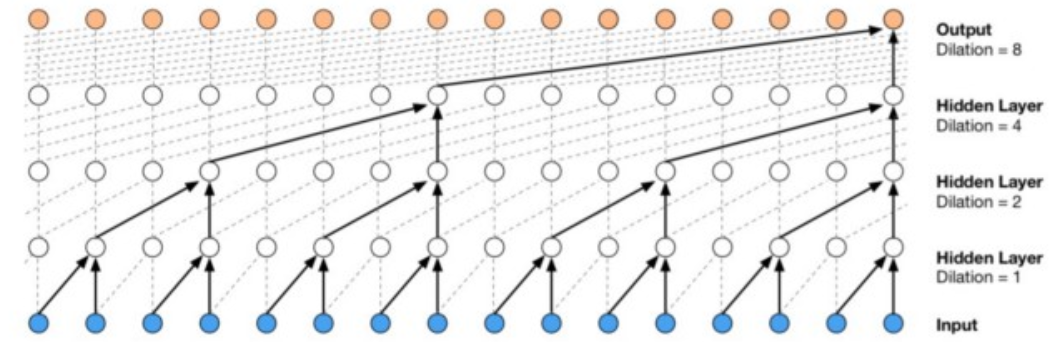
\includegraphics[width=14cm]{figures/wavenet.png}
	\end{center}

	\blfootnote{
		\fullcite{oord2016wave}
	}

\end{frame}

\begin{frame}
	\frametitle{Convolutional vs Recurrent Architectures}

	In practice, there are empirical works demonstrating the superiority of both.

	\medskip

	\begin{center}
		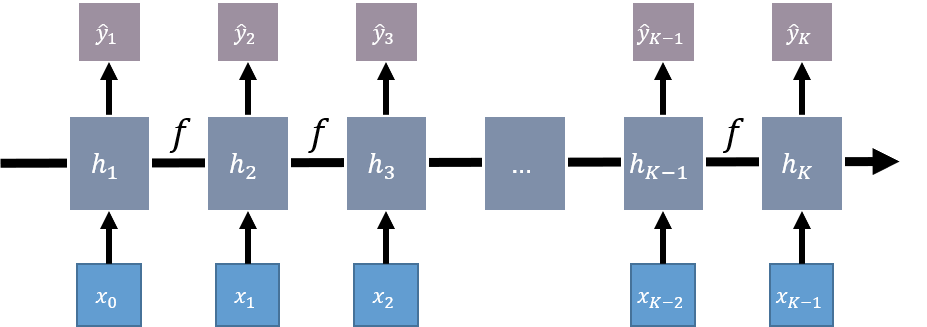
\includegraphics[width=6cm]{figures/recurrent_structure.png}
		\quad
		\textbf{v.s.}
		\quad
		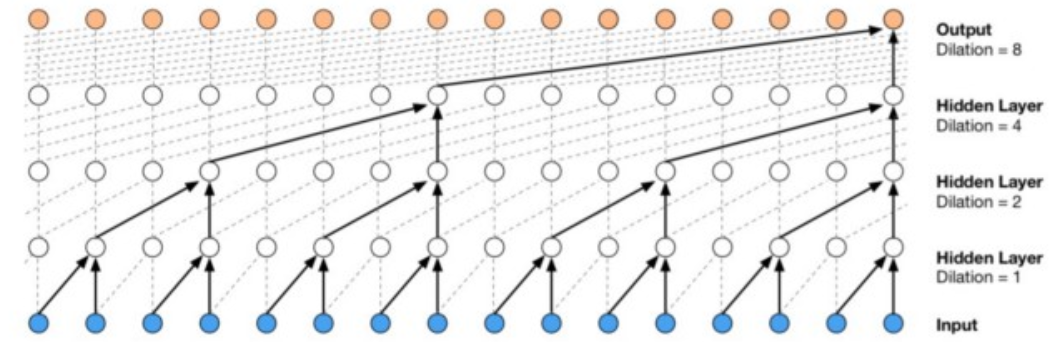
\includegraphics[width=6cm]{figures/wavenet.png}
	\end{center}

    \begin{empheq}[box=\mymath]{gather*}
	\text{
			Is one really better than the other?
	} \\
		\text{
			When should we use convolutional and recurrent architectures?
		}
    \end{empheq}

\end{frame}


\begin{frame}
	\frametitle{The Dilated Convolutional Architecture}

	For discrete sequences, define the dilated convolution operation
	\begin{equation*}
		({\bm{x}} \Conv{}_{\ell} {\bm{w}})(t)
		=
		\sum_{s \in \Z}
		{x}(s)^\tp
		{w}(t- \ell s)
	\end{equation*}

	\pause{}

	The \alert{(dilated) CNN architecture} is
	\begin{equation*}
		\begin{aligned}
			\bm h_{0,i} &= \bm x_i\\
			\bm h_{k+1,i} &= \sigma \left(\sum_{j=1}^{M_k} {\bm w}_{kji} *_{d_k} \bm h_{k,j} \right)\\
			\bm {\hat y} &= \bm h_{K,1}
		\end{aligned}
		\quad
		\begin{tabular}{ll}
			\toprule
			$\bm h_{k,i}$ & hidden state at layer $k$, channel $i$ \\
			$\bm w_{kji}$ & size $\R^l$ convolutional filters \\
			$K$           & \# layers \\
			$M_k$	      & \# channels at layer $k$ \\
			$d_k$ 		  & dilation rate at layer $k$ \\
			\bottomrule
		\end{tabular}
	\end{equation*}
\end{frame}

\begin{frame}
	\frametitle{Linear Convolutional Hypothesis Space}

	As before, turn to linear case $\sigma = \id$ and choose $d_k = l^k$, then
	\begin{equation*}
		\begin{aligned}
			\hcnn^{(l,K,\set{M_k})}
			:=
			\left\{
				\bm x \mapsto \wh{\bm y}
				:
				\bm w_{kji} \in \R^l
			\right\}
		\end{aligned}
		\qquad
		% \begin{aligned}
		\scriptsize
		\begin{cases}
			\bm h_{0,i} = \bm x_i\\
			\bm h_{k+1,i} = \sum_{j=1}^{M_k} {\bm w}_{kji} *_{d_k} \bm h_{k,j} \\
			\bm {\hat y} = \bm h_{K,1}
		\end{cases}
		\normalsize
			% &\bm h_{0,i} = \bm x_i\\
			% &\bm h_{k+1,i} = \sigma \left(\sum_{j=1}^{M_k} {\bm w}_{kji} *_{d_k} \bm h_{k,j} \right)\\
			% &\bm {\hat y} = \bm h_{K,1}
		% \end{aligned}
	\end{equation*}
	with total \# variables $m = l \sum_{k} M_{k}M_{k+1}$

	The full CNN hypothesis space is
	\begin{equation*}
		\hcnn\depen{l} =
		\bigcup_{K \in \mathbb N_+}
		\bigcup_{\set{M_k} \in \mathbb N_+^K}
		\hcnn\depen{l,K,\set{M_k}}.
	\end{equation*}
\end{frame}

\begin{frame}[c]
	\frametitle{Approximation Guarantee (Density)}

	\begin{alertblock}{Theorem [JLL, 2021]}
		Let $\{ \Htar_t : t\in\R \}$ be a family of continuous,
		linear, causal, and time-homogeneous functionals on $\ell^2(\Z,\R^d)$.
		Then, for any $\epsilon > 0$ there exists
		$\wh{\bm H} = \{ \wh{H}_t : t\in \R \} \in \hcnnl$ such that
		\begin{equation*}
			% \sup_{t\in\Z}
			% \| \Htar_t - \wh{H}_t \|
			\| \bm \Htar - \wh{\bm H} \|
			\equiv
			\sup_{t\in\Z}
			\sup_{\| \*x \|_{\ell^2} \leq 1}
			|
			\Htar_t(\*x) - \wh{H}_t(\*x)
			|
			\leq \epsilon.
		\end{equation*}
	\end{alertblock}

	\blfootnote{
		\fullcite{jiang2021approx}
	}

\end{frame}


\begin{frame}
	\frametitle{Principles of CNN Approximation}

	How does CNN approximation work?

	\begin{itemize}[<+->]
		\item Target
		\begin{equation*}
			\Htar_t(\bm x)
			=
			\sum_{s = 0}^{\infty}
			\rho^{(\bm H^*)}(s)^\tp
			x(t-s)
			\qquad
			\text{(Riesz Representation)}
		\end{equation*}
		\item CNN Approximation
		\begin{equation*}
			\begin{aligned}
				\wh{H}_t(\bm x)
				=
				\sum_{s = 0}^{l^K - 1}
				\wh{\rho} (s)^\tp
				x(t-s)
				\qquad
				\wh{\bm \rho}
=
				\sum_{\text{all channels}}
				{\bm w_{K-1}}
				\Conv{}_{l^{K-1}}
				{\bm w_{K-2}}
				\Conv{}_{l^{K-2}}
				\cdots
				\Conv{}_{l^{2}}
				{\bm w_{1}}
				\Conv{}_{l^{1}}
				{\bm w_{0}}
				% \sum_{i_0,1,i_{K-1}}
				% {\bm w}_{K-1,i_{K-1},1}
				% \Conv{}_{l^{K-1}}
				% {\bm w}_{K-2,i_{K-2},i_{K-1}}
				% \Conv{}_{l^{K-2}}
				% \cdots
				% \Conv{}_{l^2}
				% {\bm w}_{1,i_{1},i_{2}}
				% \Conv{}_{l}
				% {\bm w}_{0,i_{0},i_{1}}
			\end{aligned}
		\end{equation*}
		\item
		Error consists of two parts
		\begin{equation*}
			\sup_{\|\bm x\|_{\ell^2} \leq 1}
			| \Htar_t(\bm x) - \wh{H}_t(\bm x) |^2
			\leq
			\underbrace{
				\sum_{s=0}^{l^{K}-1}
				\| \rho^{(\bm H^*)}(s) - \wh{\rho}(s) \|^2
			}_{
				\text{representation by convs}
			}
			+
			\underbrace{
				\sum_{s=l^K}^{\infty}
				\| \rho^{(\bm H^*)}(s) \|^2
			}_{
				\text{tail (memory) $\rightarrow$ 0}
			}
		\end{equation*}
	\end{itemize}

\end{frame}

\begin{frame}
	\frametitle{Tensorization Rank}

	What ${\bm \rho^{(\bm H)}}$ can be efficiently represented by deep dilated convolutions?

	\begin{itemize}[<+->]
		\item
		Let us take $d=1$, $l=K=2$. Then, we need the convolution filters to represent the first $l^K = 4$ indices of $\bm \rho^{(\bm H)}$.
		\item
		Define the tensorization procedure
		\begin{equation*}
			T(
				{\bm \rho}^{(\bm H)}_{[0,3]}
			)
			=
			\begin{pmatrix}
				{\bm \rho}^{(\bm H)}_{0} &
				{\bm \rho}^{(\bm H)}_{1} \\
				{\bm \rho}^{(\bm H)}_{2} &
				{\bm \rho}^{(\bm H)}_{3}
			\end{pmatrix}
		\end{equation*}
		\item
		If we use 1 channel, we have
		\begin{equation*}
			\wh{\bm \rho}
			= {\bm w_2} \Conv{}_{2} {\bm w_1}
			\qquad
			T(
				\wh{\bm \rho}
			)
			=
			\begin{pmatrix}
				w_{11} \\
				w_{12}
			\end{pmatrix}
			\begin{pmatrix}
				w_{21} &
				w_{22}
			\end{pmatrix}
		\end{equation*}
		\item
		Hence, approximation error is that of the best rank-1 approximation of
		$T({\bm \rho}^{(\bm H)}_{[0,3]})$, i.e. tail sum of singular values
		due to the \alert{Eckart-Young-Mirsky theorem}
	\end{itemize}

\end{frame}

\begin{frame}
	\frametitle{Approximation Rates by CNNs}

	This motivates us to define the complexity measure
	\small
	\begin{equation*}
		C\depen{l,g}(\bm H)
		=
		\inf
		\Bigg\{
			c:
			(
				\Sigma_{i=s+K}^{lK}
				\underbrace{
					(\sigma_i\depen{K})^2
				}_{
					\mathclap{\text{tail of singular values of tensorization}}
				}
			)^{\frac 1 2}
			\leq c
			\overbrace{g(s)}^{
				\text{decay rate}
			}
			,
			~s\geq 0, K\in \mathbb N_+\Bigg
		\}
	\end{equation*}
	\normalsize
	% \begin{equation*}
	% 	C^{(l,g)}
	% 	=
	% 	\inf
	% 	\left\{
	% 		c :
	% 	\right\}
	% \end{equation*}

	\begin{alertblock}{Theorem [JLL, 2021]}
		Let $\{ \Htar_t : t\in\R \}$ be a family of continuous,
		linear, causal, and time-homogeneous functionals on $\ell^2(\Z,\R^d)$.
		Let $l\geq 2$ and $g\in c_0(\mathbb{N}, \R_+)$.
		Then, for any ${\bm H^*}$ we have
		\begin{equation*}
			\inf_{\wh{\bm H} \in \hcnn^{(l,K,\{M_k\})}}
			\| {\bm H^*} - {\wh{\bm H}} \|
			\leq
			d g(K M^{\frac{1}{K}} - K) C^{(l,g)}(\bm H^*)
			+
			\| {{\bm \rho}_{[l^K,\infty]}^{\bm H^*}} \|_2
		\end{equation*}
		where
		$M = (\Sigma_{k=2}^{K}M_k M_{k-1}-lK)/d$.
	\end{alertblock}

	\blfootnote{
		\fullcite{jiang2021approx}
	}

\end{frame}


\begin{frame}
	\frametitle{Convolutional vs Recurrent Achitectures}

	So, is $\hrnn$ or $\hcnn$ better? In general, neither!

    \begin{empheq}[box=\mymath]{equation*}
		\textbf{Insight:}
		\qquad
		\begin{aligned}
			&\text{
				RNN works well if ${\bm \rho}^{\bm H^*}$ decays exponentially
			} \\
			&\text{
				CNN works well if ${\bm \rho}^{\bm H^*}$ has low rank under tensorization
			}
		\end{aligned}
    \end{empheq}

	\begin{center}
		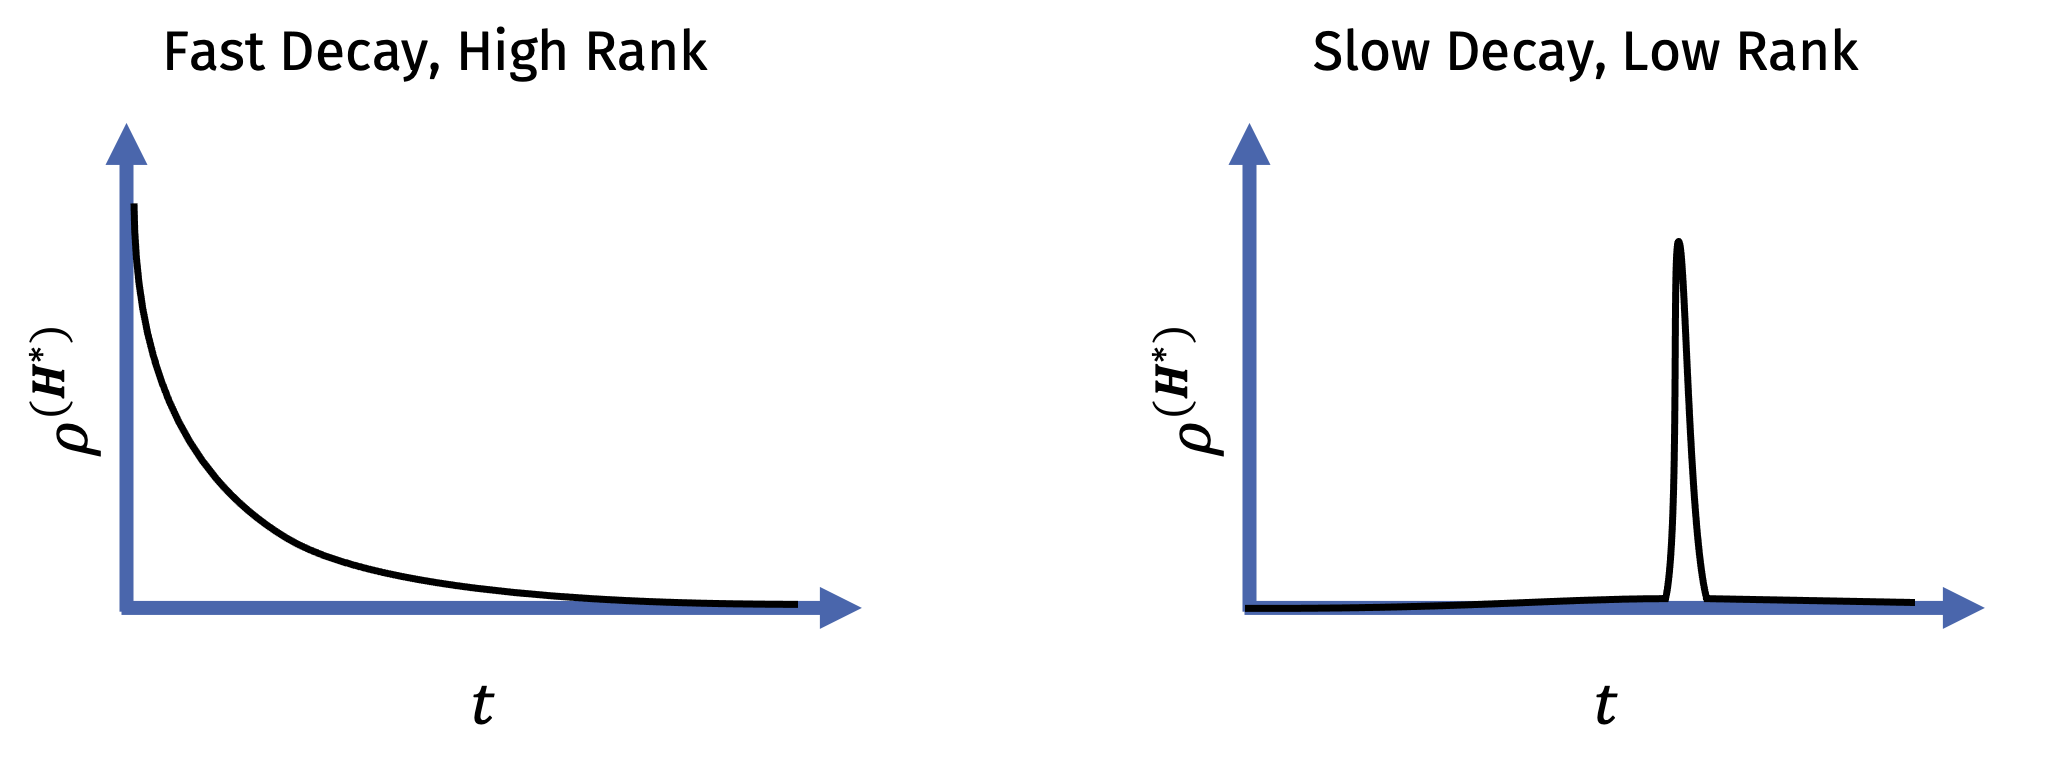
\includegraphics[width=0.9\textwidth]{figures/rnn_vs_cnn.png}
	\end{center}

\end{frame}

    \section{Encoder-Decoder Architectures}

\begin{frame}
	\frametitle{Encoder-Decoder Architectures for Modelling Sequences}

	Alternative to RNNs and CNNs are \alert{encoder-decoder} class of
	architectures

	\begin{center}
		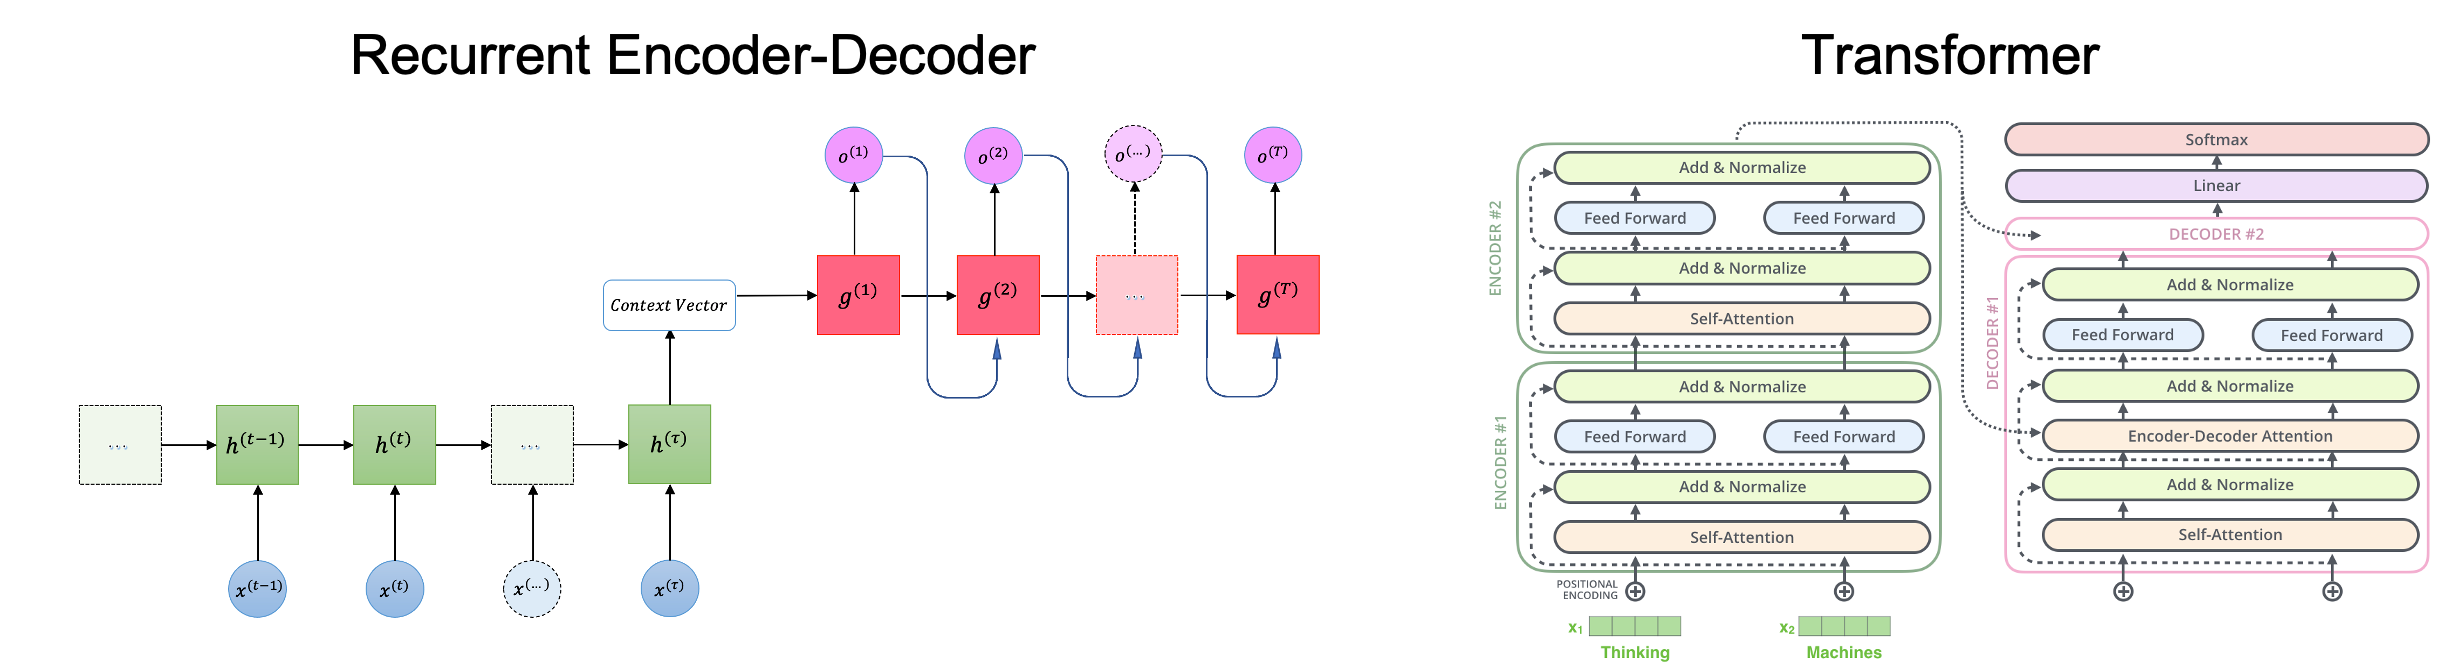
\includegraphics[width=\textwidth]{figures/ed_transf.png}
	\end{center}


    \begin{empheq}[box=\mymath]{gather*}
        \text{
			How do they compare with RNN and CNN?
        }
    \end{empheq}

\end{frame}

\begin{frame}
	\frametitle{Linear Recurrent Encoder-Decoder}

	\begin{center}
		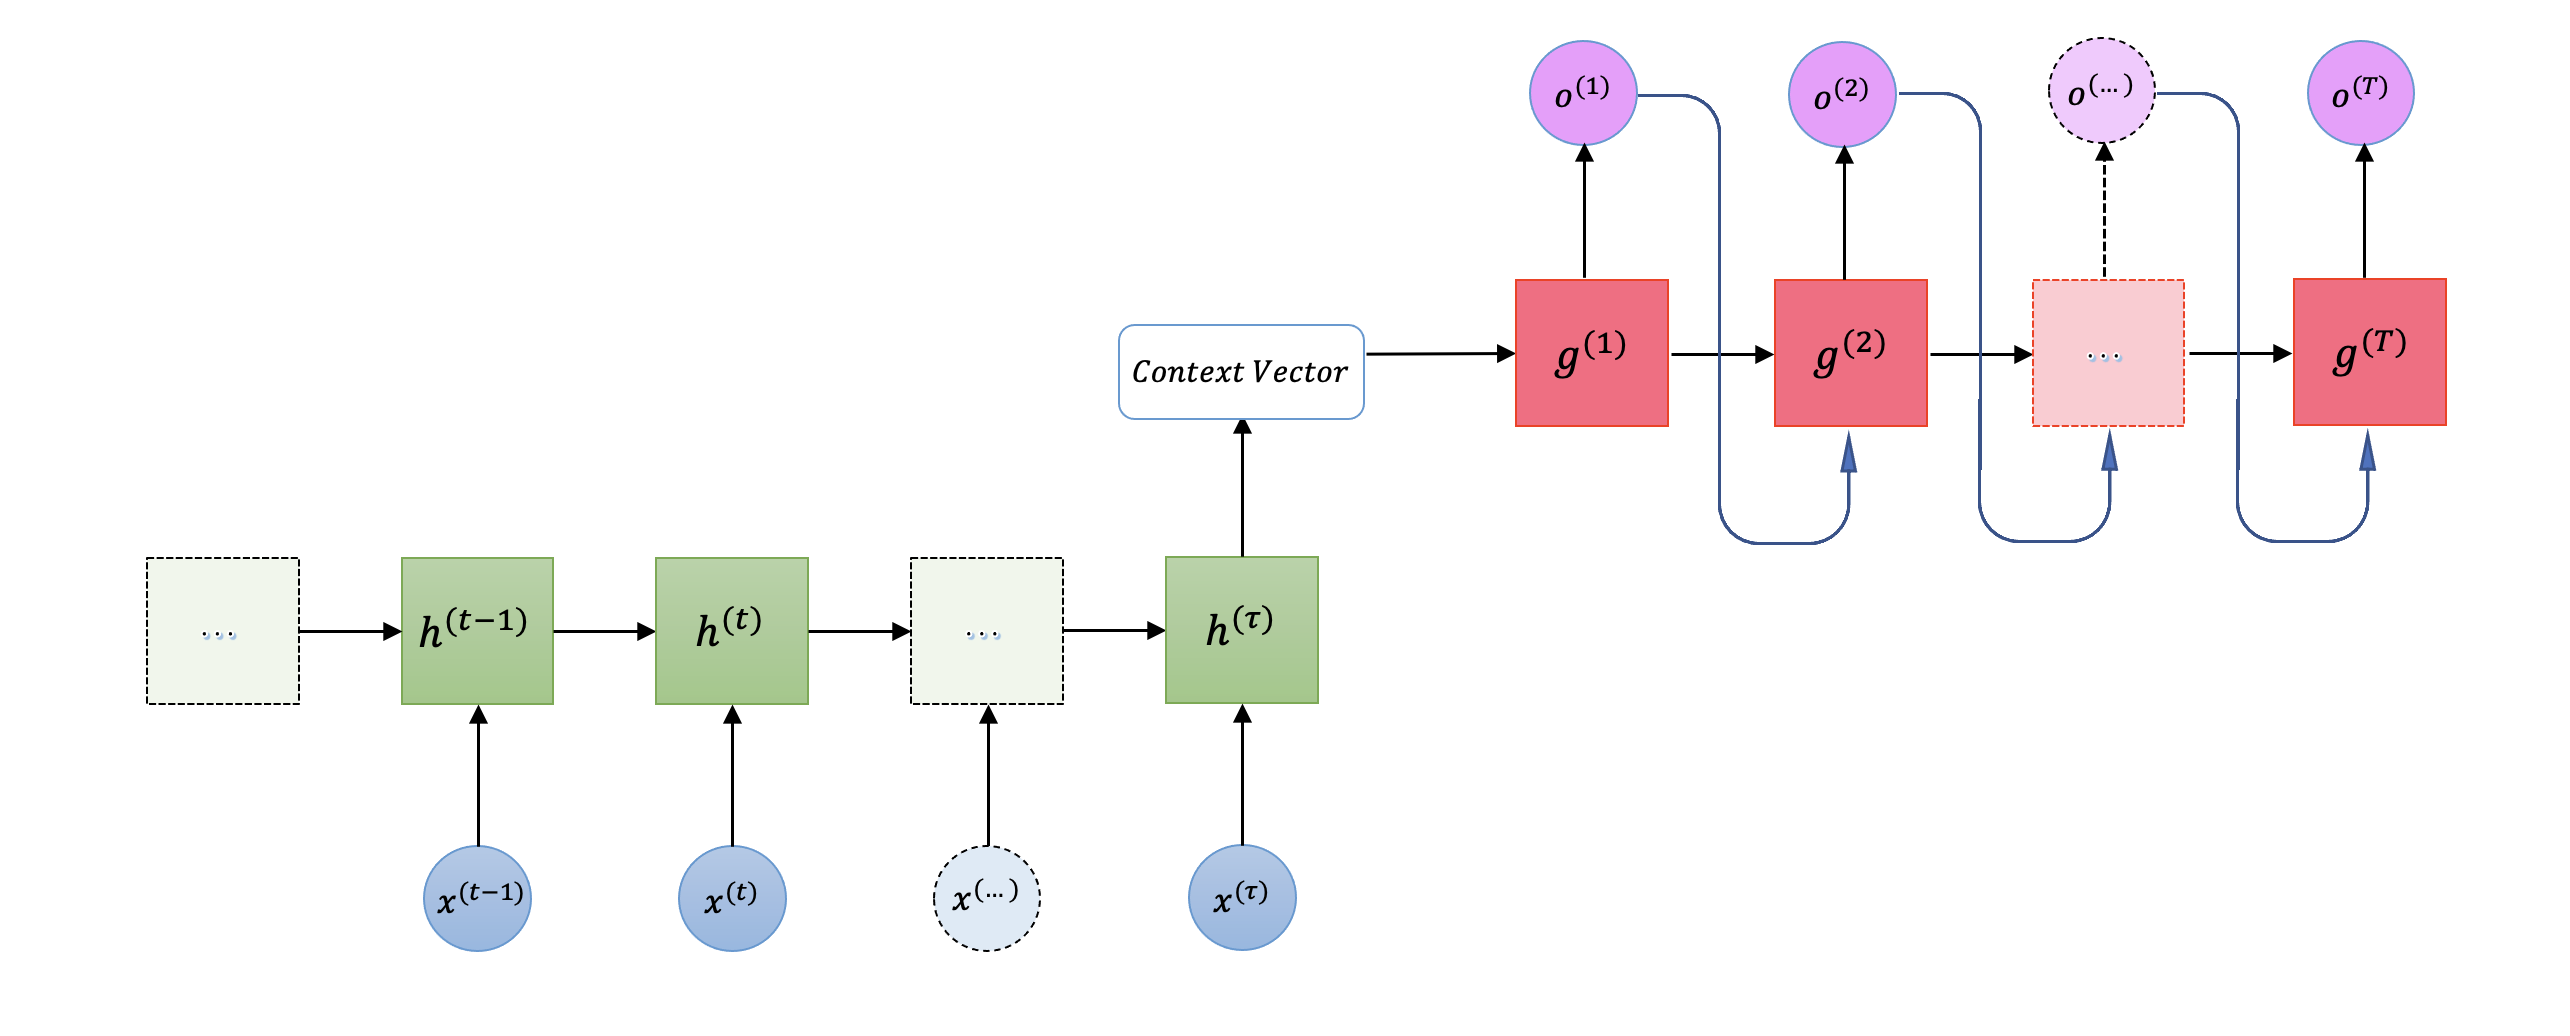
\includegraphics[width=0.8\textwidth]{figures/encdec.png}
	\end{center}

	As before, linear continuous variant gives the following dynamics
	\begin{equation*}
		\begin{matrix}
			\dot{h}_s = Wh_s+Ux_s,
			& v=Qh_0,
			& s\leq 0,
			& h_s \in \R^{m_E}, v \in \R^{N}\\
			\dot{g}_t = Vg_t,
			& g_0=Pv,
			&
			& g_t \in \R^{m_D}
			\\
			y_t = c^\top g_t,
			&
			& t\ge 0
			&
		\end{matrix}
	\end{equation*}
	% \begin{equation*}
	% 	\begin{aligned}
	% 		\dot{h}_s
	% 		& = Wh_s+Ux_s,
	% 		&& v=Qh_0, \quad &s\leq 0,
	% 		&&h_s \in \R^{m_E},
	% 		v \in \R^{N}
	% 		\\
	% 		\dot{g}_t
	% 		& = Vg_t,
	% 		&& g_0=Pv,
	% 		&& g_t \in \R^{m_D}
	% 		\\
	% 		y_t
	% 		&=c^\top g_t,
	% 		&&
	% 		&&t\ge 0,
	% 		% &V\in\mathbb R^{m_D\times m_D}, U\in\mathbb R^{m_E\times d},\\
	% 		% Q\in\mathbb R^{N\times m_E}, & P\in\mathbb R^{m_D\times N}.
	% 	\end{aligned}
	% \end{equation*}

\end{frame}

\begin{frame}
	\frametitle{Linear Recurrent Encoder-Decoder Hypothesis Space}

	The hypothesis space is
	\begin{equation*}
		\henc^{(m_E,m_D,N)} :=
		\Big\{\bhh: \hat H_t = \int_{0}^{\infty} c^\top e^{Vt} PQe^{W s} U x_{t-s} ds \Big\}
	\end{equation*}
	and
	\begin{equation*}
		\henc := \bigcup_{N,m_E,m_D \in \mathbb{N}_+}
		\henc^{(m_E,m_D,N)}
	\end{equation*}

	\pause{}

	\medskip
	\medskip

	\begin{empheq}[box=\mymath]{gather*}
		\text{
			How is this different from RNN/CNN?
		}
    \end{empheq}

\end{frame}

\begin{frame}
	\frametitle{Approximation Guarantee (Density)}

	\begin{alertblock}{Theorem [LJL, 2022]}
		Let $\{ \Htar_t : t\in\R \}$ be a family of continuous,
		linear, \sout{causal}, regular and \sout{time-homogeneous} functionals
		on $C_0(\R,\R^d)$.
		Then, for any $\epsilon > 0$ there exists $\{ \wh{H}_t : t\in \R \} \in \henc$ such that
		\begin{equation*}
			\| \bm \Htar - \wh{\bm H} \|
			% \sup_{t\in\R}
			% \| \Htar_t - \wh{H}_t \|
			\equiv
			\sup_{t\in\R}
			\sup_{\| \*x \|_C \leq 1}
			|
			\Htar_t(\*x) - \wh{H}_t(\*x)
			|
			\leq \epsilon.
		\end{equation*}
	\end{alertblock}

	Main idea: Riesz representation for non-time-homogeneous functional
	\begin{equation*}
		H^*_t(\*x) =
		\int_{0}^{\infty}
		x_{t-s}^\tp \rho(t,s) ds
	\end{equation*}
	Then, recurrent encoder-decoder approximates $\rho(t,s)$ by
	$c^\top e^{Vt} PQe^{W s} U$


	\blfootnote{
		\fullcite{li2021approxed}
	}
\end{frame}

\begin{frame}
	\frametitle{The Temporal Product Structure}

	Notice that recurrent encoder-decoder approximates
	\begin{equation*}
		\rho^{(\bm H^*)}(t,s)
		\qquad
		\rightarrow
		\qquad
		\underbrace{
			c^\top e^{Vt}P
		}_{
			{\bm \phi}(t)
		}
		\cdot
		\underbrace{
			Qe^{W s} U
		}_{
			{\bm \psi}(s)
		}
		=
		\sum_{n=1}^{N}
		\phi_n(t) \psi_n(s)
	\end{equation*}
	\begin{itemize}[<+->]
		\item
		Hence, $N$ can be taken small if ${\bm \rho}^{\bm H^*}$
		is of a \alert{temporal product structure}, i.e.
		having low effective rank under functional SVD
		(Proper Orthogonal Decomposition, POD)!
		\item
		This leads to precise approximation rates in terms of
		$\{m_E, m_D,N\}$ \refhl{[LJL, 2022]}
	\end{itemize}


	\blfootnote{
		\fullcite{li2021approxed}
	}
\end{frame}

\begin{frame}
	\frametitle{Low vs High (Effective) Rank Relationships}

	\begin{center}
		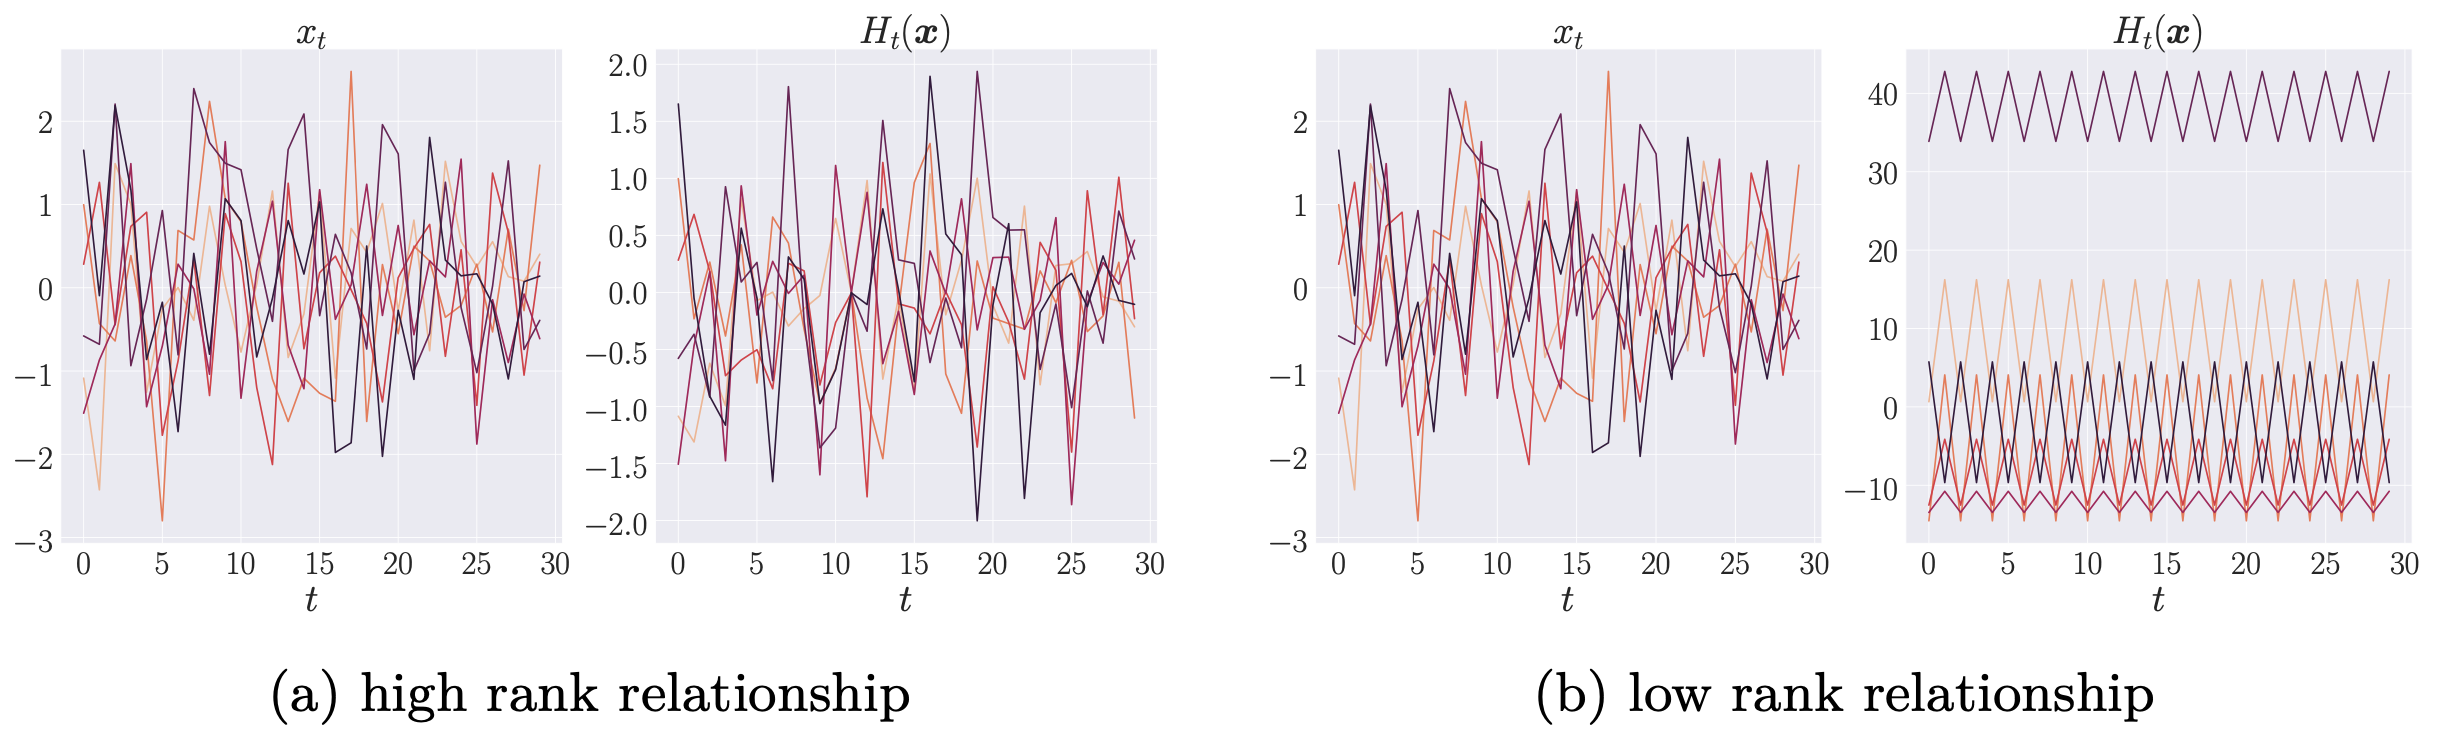
\includegraphics[width=\textwidth]{figures/low_high_rank.png}
	\end{center}

	\begin{empheq}[box=\mymath]{equation*}
		\textbf{Insight:}
		\qquad
		\begin{aligned}
			&\text{
				Encoder-decoders are most effective in capturing
			}\\
			&\text{
				temporal product structures with low effective rank!
			}
		\end{aligned}
    \end{empheq}

\end{frame}

    \begin{frame}
	\frametitle{Summary}

	We introduced a basic mathematical setting that allows
	precise analysis (in the linear setting)
	of three architectures for sequence modelling
	\begin{itemize}
		\item RNN, CNN, Recurrent Encoder-Decoder
	\end{itemize}

	From the approximation viewpoint
	\begin{itemize}
		\item Can all achieve density in appropriate functional spaces
		\item Efficient approximation depends on different notions of complexity
		\begin{itemize}
			\item RNN: Exponential memory decay
			\item CNN: Low rank under tensorization
			\item Recurrent Encoder-Decoder:
			Low rank under temporal products
		\end{itemize}
	\end{itemize}

	\begin{empheq}[box=\mymath]{gather*}
		\text{
			Need \alert{structural compatibility}
			between the model and the target
		}
    \end{empheq}

\end{frame}

\begin{frame}
	\frametitle{References}

	\begin{enumerate}
		\item
		\fullcite[]{li2020onthe}
		\item
		\fullcite[]{jiang2021approximation}
		\item
		\fullcite[]{li2022approxlinear}
		\item
		\fullcite[]{li2021approxed}
		\item
		\fullcite[]{li2022deep}
	\end{enumerate}


\end{frame}

    \begin{frame}[focus]
        Thank you!
    \end{frame}

\end{document}
